\documentclass[a4paper, 12pt]{book}
%\usepackage[active]{srcltx}
\usepackage[czech]{babel}
\usepackage[utf8]{inputenc}

\usepackage{amsmath}
\usepackage{amsfonts}
\usepackage{amssymb}
\usepackage{amsthm}
\usepackage{mathtools} % needs texlive-latex3 package (Ubuntu)

\usepackage{graphicx}
\usepackage{hyperref}
\hypersetup{backref,colorlinks=true, raiselinks=true}
%
\theoremstyle{definition}
\newtheorem{theorem}{Věta}[section]
\newtheorem{proposition}[theorem]{Tvrzení}
\newtheorem{definition}[theorem]{Definice}
\newtheorem{remark}[theorem]{Poznámka}
\newtheorem{lemma}[theorem]{Lemma}
\newtheorem{corollary}[theorem]{Důsledek}
\newtheorem{example}[theorem]{Příklad}
\newtheorem{exercise}[theorem]{Cvičení}

%\numberwithin{equation}{document}
%
\def\div{{\rm div}}
\def\Lapl{\Delta}
\def\grad{\nabla}
\def\supp{{\rm supp}}
\def\dist{{\rm dist}}
%\def\chset{\mathbbm{1}}
\def\chset{1}
%
\def\Tr{{\rm Tr}}
\def\to{\rightarrow}
\def\weakto{\rightharpoonup}
\def\imbed{\hookrightarrow}
\def\cimbed{\subset\subset}
\def\range{{\mathcal R}}
\def\leprox{\lesssim}
\def\argdot{{\hspace{0.18em}\cdot\hspace{0.18em}}}
\def\Distr{{\mathcal D}}
\def\calK{{\mathcal K}}
\def\FromTo{|\rightarrow}
\def\convol{\star}
\def\impl{\Rightarrow}
\DeclareMathOperator*{\esslim}{esslim}
\DeclareMathOperator*{\esssup}{ess\,supp}
\DeclareMathOperator{\ess}{ess}
\DeclareMathOperator{\osc}{osc}
\DeclareMathOperator{\curl}{curl}
\DeclareMathOperator{\cotg}{cotg}
\def\Lin{\mathit{Lin}}
\def\dx{\d x}
%
%\def\Ess{{\rm ess}}
%\def\Exp{{\rm exp}}
%\def\Implies{\Longrightarrow}
%\def\Equiv{\Longleftrightarrow}
% ****************************************** GENERAL MATH NOTATION
\def\Real{{\rm\bf R}}
\def\Rd{{{\rm\bf R}^{\rm 3}}}
\def\RN{{{\rm\bf R}^N}}
\def\D{{\mathbb D}}
\def\Nnum{{\rm\bf N}}
\def\Qnum{{\rm\bf Q}}
\def\Measures{{\mathcal M}}
\def\d{\,{\rm d}}               % differential
\def\sdodt{\genfrac{}{}{}{1}{\rm d}{{\rm d}t}}
\def\dodt{\genfrac{}{}{}{}{\rm d}{{\rm d}t}}
%
\def\vc#1{\mathbf{\boldsymbol{#1}}}     % vector
\def\tn#1{{\mathbb{#1}}}    % tensor
\def\abs#1{\lvert#1\rvert}
\def\Abs#1{\bigl\lvert#1\bigr\rvert}
\def\bigabs#1{\bigl\lvert#1\bigr\rvert}
\def\Bigabs#1{\Big\lvert#1\Big\rvert}
\def\ABS#1{\left\lvert#1\right\rvert}
\def\norm#1{\bigl\Vert#1\bigr\Vert} %norm
\def\close#1{\overline{#1}}
\def\inter#1{#1^\circ}
\def\eqdef{\mathrel{\mathop:}=}     % defining equivalence
\def\where{\,|\,}                    % "where" separator in set's defs
\def\timeD#1{\dot{\overline{{#1}}}}
%
% ******************************************* USEFULL MACROS
\def\RomanEnum{\renewcommand{\labelenumi}{\rm (\roman{enumi})}}   % enumerate by roman numbers
\def\rf#1{(\ref{#1})}                                             % ref. shortcut
\def\prtl{\partial}                                        % partial deriv.
\def\Names#1{{\scshape #1}}
\def\rem#1{{\parskip=0cm\par!! {\sl\small #1} !!}}
\def\vysl#1{\par$[$ #1 $]$}
\def\df#1{\emph{#1}}
\def\todo#1{{\color{green}TODO:} #1}

%\newenvironment{pmatrix*}[1][\unskip]{\left(\begin{array}[ #1]}{\end{array}\right)}

%
%
% ******************************************* DOCUMENT NOTATIONS
% document specific
%***************************************************************************
%
\addtolength{\textwidth}{2cm}
\addtolength{\vsize}{2cm}
\addtolength{\topmargin}{-1cm}
\addtolength{\hoffset}{-1cm}
\begin{document}
\parskip=2ex
\parindent=0pt

\tableofcontents


\chapter{Motivační praktické problémy}
\section{Fyzikální motivace}
\subsection{Aerodynamická brzda - separace proměnných}
Na jednoduché fyzikální úloze si připomeneme pojmy pro jednoduché obyčejné diferenciální rovnice
a dvě základní metody jejich řešení.
Auto s počáteční rychlostí $v_0=100$ km za hodinu jede s vyřazeným motorem. Při vysokých 
rychlostech převažuje aerodynamický odpor a odporová síla je úměrná druhé mocnině rychlosti.
Máme určit průběh rychlosti jako funkci času. 

Použitím druhého Newtonova zákona dostaneme pro zpomalený pohyb rovnici:
% připomenutí ODR
\begin{equation}
  \label{eq:brzda}
  m\frac{\d v}{\d t}(t) = -k v^2(t),\qquad v(0)=v_0=100,
\end{equation}
kde $m$ je hmotnost vozidla, $t$ je čas a $k$ je vhodná konstanta závisející na tvaru vozidla.
Řešením rovnice je funkce $v(t)$ přičemž $v$ se nazývá \df{závisle proměnná} a $t$ \df{nezávisle proměnná}.
V rovnici \eqref{eq:brzda} se vyskytuje nejvýše první derivace hledané funkce $v(t)$, proto se jedná 
o \df{rovnici prvního řádu}. Na pravé straně je nelineární funkce $f(v)= cv^2$ závisle proměnné, proto se jedná o \df{nelineární diferenciální rovnici}.
Jelikož pravá strana nezávisí přímo na nezávislé proměnné, jedná se o tzv. \df{autonomní rovnici}.

Pro řešení nelineárních diferenciálních rovnic neexistuje řádný univerzální postup, do\-kon\-ce pro většinu rovnic nelze nalézt analytické řešení.
Rovnice \eqref{eq:brzda} umožňuje řešení pomocí \df{separace proměnných}. Derivaci napíšeme jako podíl diferenciálů a rovnici upravíme do tvaru, kde 
na levé straně je pouze závisle proměnná a na pravé pouze nezávisle proměnná, tedy
\[
    v^{-2} \d v =  \alpha \d t, \quad \alpha = -k/m 
\]
Nyní obě strany vyintegrujeme, pozor na integrační konstantu $C$,
\[
    -v^{-1} = \int v^{-2}\; \d v = \int \alpha\; \d t =\alpha t + C.
\]    
A vyjádříme $v$:
\[
    v(t) = \frac{-1}{\alpha t + C}
\]
Pro určení konstanty $C$ použijeme \df{počáteční podmínku} $v(0) = v_0 = 100$,
\[
  C = -v^{-1} - \alpha t = -v_0^{-1}
\]
a celkový výsledek je tedy:
\[
  v(t) = \frac{v_0}{1-\alpha tv_0}.
\]



\subsection{Rozjezd auta - variace konstant}
V případě lineárních rovnic se autonomním rovnicím říká \df{homogenní} a lze je vždy řešit separací. Pokud se na pravé straně navíc objeví člen
zavislý pouze na čase, \df{absolutní člen}, jedná se o \df{nehomogenní rovnici}, kterou řešíma \df{variací konstant}.

Uvažujme zrychlený pohyb, kde v čase lineárně zvyšujeme výkon motoru a zároveň uvažujeme odporovou sílu přímo úměrnou rychlosti:
\[
  mv'(t) = Pt - c v(t), \qquad v(0)=0
\]
Jedná se o lineární rovnici, protože obsahuje pouze členy obsahující závisle proměnnou $v$ nebo její derivaci $v'$. Absolutní člen $Pt$ by mohl být i nelineární,
např. $Pt^2$, a stále by šlo o lineární rovnici. Lineární rovnice obvykle zapisujeme tak, aby na levé straně byly členy obsahující závislou proměnnou a na pravé straně je buď nula (homogenní rovnice),
nebo \uv{absolutní člen}, kterému se v kontextu lineárních rovnic obvykle říká \df{pravá strana}.

Nejprve vyřešíme homogenní rovnici $mv'= - cv$, pomocí separace proměnných najdeme řešení $ v=Ce^{-\alpha t}$, $\alpha = c/m$. Nyní hledáme řešení původní rovnice ve tvaru:
\[
   v(t) = C(t) e^{-\alpha t}
\]
kde jsme provedli \uv{variaci} integrační konstanty $C$. Neúplné řešení v tomto tvaru do\-sa\-dí\-me do nehomogenní rovnice:
\[
  m C'(t) e^{-\alpha t} - m \alpha C(t) e^{-\alpha t} = Pt - m \alpha C(t) e^{-\alpha t}
\]
oba poslední členy se odečtou, dále vyjádříme $C'$ a integrujeme per partes:
\[
  C(t) = \frac{P}{m} \int te^{\alpha t} \; \d t = \frac{P}{m\alpha^2}\left(\alpha t - 1\right)e^{\alpha t} + C_0.
\]
Celé řešení je pak
\[
  v(t) = C(t) e^{-\alpha t} = C_0 e^{-\alpha t} + \frac{P}{m\alpha^2} (\alpha t - 1)
\]
přičemž $C_0$ se opět určí z počáteční podmínky. Všimněme si, že počáteční podmínka ovlivňuje jen první člen řešení, který odpovídá řešení 
homogenní rovnice, druhý člen, kterému se říká \df{partikulární řešení} na počáteční podmínce nezávisí, ale závisí na absolutním členu. 


\subsection{Tlumený a buzený oscilátor}
\label{sec::oscilator}
V mnoha aplikacích je třeba vyšetřovat různé oscilující systémy. Může jít o~mechanické oscilátory jako v~případě 
vibrací různých motorů, nebo o~elektrický oscilátor (RLC obvod), nebo o~model visko-elastického materiálu (elastická plastelína), nebo o~gravitační oscilátor (kyvadlo).
\begin{figure}[h]
\label{fig:oscilator}
\begin{center}
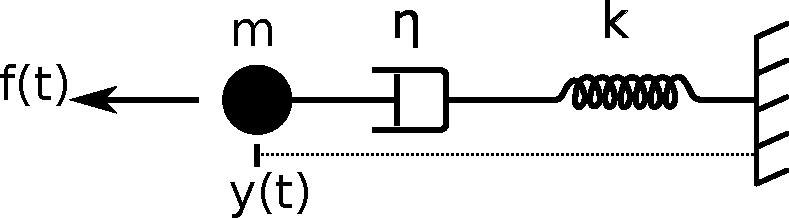
\includegraphics[scale=0.4]{maxwell_diagram.pdf}
\caption{Schéma tlumeného oscilátoru.}
\end{center}
\end{figure}
Tlumený a~buzený oscilátor (viz. schéma \ref{fig:oscilator}) se skládá z~pružiny o~tuhosti $k$ (závislost síly na výchylce $y$),
sériově zapojeného tlumiče o~dynamické tuhosti $\eta$ (závislost síly na rychlosti změny výchylky) a~tělesa o~hmotnosti $m$, které je \emph{buzeno} vnější silou $f(t)$
(obvykle periodickou). 
Použitím druhého Newtonova zákona a~bilance sil dostaneme rovnici:
\[
 m\frac{\d^2y}{\d t^2}+\eta \frac{\d y}{\d t}+ky=f(t),\quad t>0,\quad y(0)=y_0,\quad \frac{\d y}{\d t}(0) = y_1,
\]
kterou můžeme zjednodušit na tvar:
\[
  y'' + \alpha y' + \beta y = F(t),\quad \alpha=\frac{\eta}{m},\quad  \beta=\frac{k}{m},\quad F(t)=\frac{f(t)}{m}
\]

Jedná se o nehomogenní (pokud $f\ne 0$) lineární rovnici druhého řádu. Při\-po\-meň\-me obvyklou metodu řešení takovéto rovnice.
Nejprve řešíme \df{charakteristickou rovnici}
\[
  Y^2 + \alpha Y + \beta =0.
\]
Tato kvadratická rovnice má buď jeden (násobný) nebo dva (obecně komplexní) kořeny $Y^+$, $Y^-$, pak má homogenní rovnice ($F=0$) řešení ve tvaru
\begin{equation}
   \label{eq:charakteristicka}
   y(t) = C^{+}e^{Y^{+} t} + C^{-}e^{Y^{-} t}.
\end{equation}
Pro reálné kořeny (převaha tlumení) máme prostý součet dvou exponenciel. Pro násobný kořen $Y$ je řešení ve tvaru
\[
  y(t) = C_1 t e^{Yt} + C_2 e^{Yt}.
\]
Pro komplexně sdružené kořeny $Y_{\pm} = a \pm i b$ musí být komplexně sdružené i integrační konstanty $C^{+}$, $C^{-}$ v rovnici \eqref{eq:charakteristicka}, jelikož
řešení $y(t)$ má být reálná funkce, pak lze řešení napsat jako:
\begin{align*}
   y(t) &= (A + i B) e^{at} e^{ibt} + (A-iB)e^{at}e^{-ibt} = A e^{at} (e^{ibt} + e^{-ibt}) + B e^{at} i(e^{ibt} - e^{-ibt}) \\
   &= e^{at}\big( 2 A cos(bt) + 2 B sin(bt) \big).
\end{align*}
Pro některé speciální pravé strany $F$ existují předpisy pro partikulární řešení.

Nyní naznačíme, odkud se vzala výše ukázaná metoda řešení pomocí charakteristické rovnice, jak tato charakteristická rovnice souvisí s~charakteristickou rovnicí pro vlastní čísla matice,
a~jak lze řešit nehomogenní lineární rovnici pro obecnou pravou stranu. Klíčovým trikem, je převod rovnice vyššího řádu na soustavu rovnic nižšího řádu. Zavedeme novou proměnnou $z(t)$ pro derivaci $y'$,
pak můžeme původní rovnici napsat ve tvaru soustavy:
\begin{align}
   y'(t) - z(t) &= 0, & y(0) = y_0\\
   z'(t) + \alpha z(t) + \beta y(t) &= F(t), & z(0)= y_1
\end{align}
Tuto lineární soustavu můžme napsat ve vektorovém tvaru
\[
    \frac{\d}{\d t}    
    \begin{pmatrix}
       y \\ z
    \end{pmatrix}
    +
    \begin{pmatrix}
        0  & -1\\
        \beta & \alpha
    \end{pmatrix}
    \begin{pmatrix}
        y \\ z
    \end{pmatrix}
    =
    \begin{pmatrix}
     0 \\ F(t)
    \end{pmatrix}
\]
nebo při vhodném označení vektorů a matic ještě jednodušeji:
\[
    \vc Y'(t) + \tn A \vc Y(t) = \vc F(t).
\]
Tento vektorový zápis budeme dále hojně využívat, vektory budou vždy psány tučně, matice dvojitým fontem.



% fyzikalni vyznam pocatecnich podminek
% naznaceni souvislosti s charakteristickym polynomem

\subsection{Systém dravec-kořist}
Uvažujme jednoduchý ekologický systém složený z populace predátora  a jeho kořisti (klasickým příkladem jsou lišky a zajíci).
Označme $x(t)$ počet zajíců a $y(t)$ počet lišek v čase $t$ s počátečními velikostmi $x_0$ a $y_0$. 
Zajíci mají neomezený zdroj potravy, lišky se živí pouze lovem zajíců.
Tento ekologický systém popisuje Lotkův-Voltarrův systém diferenciálních rovnic:
\begin{align}
  \frac{\d x}{\d t} &= x(a-\alpha y), \quad x(0)=x_0\\
  \frac{\d y}{\d t} &= y(-c+\gamma x), \quad y(0)=y_0.
\end{align}
Význam členů na pravé straně je: $ax$ vyjadřuje přirozený přírůstek zajíců za jednotku času, $-\alpha xy$ umrtí zajíců v důsledku interakce,
$\gamma x y$ přírůstek lišek v důsledku interakce, $-cy$ přirozený úbytek lišek.
Označme $\vc x = (x,y)^T$ a zapišme vektorově:
\[
   \frac{\d \vc x}{\d t} = \begin{pmatrix} x'\\ y' \end{pmatrix}
   = \begin{pmatrix} a & -\alpha x \\ \gamma y & - c\end{pmatrix} 
     \begin{pmatrix} x \\ y\end{pmatrix} = \vc F(\vc x).
\]
Vidíme, že matice na pravé straně sama závisí na hledaném řešení, proto se jedná o~nelineární systém obyčejných diferenciálních rovnic prvního řádu.



\chapter{Teorie soustav ODR}
Systémy obyčejných diferenciálních rovnic (ODR) jsou základním modelem při popisu netriviálních 
časově proměnných jevů z fyziky, chemie, biologie, ekonomie, elektrotechniky a mnoha dalších oborů. 
Cílem dalších kapitol bude nejprve prozkoumání základních obecných vlastností soustav ODR (kapitola \ref{soustavy})
a poté seznámení se s řešením lineárních soustav (kapitoly \ref{linearni_soustavy} a \ref{konst_koef}). Další kapitoly budou věnovány 
úvodu do numerických metod pro řešení ODR a jejich soustav.

\section{Soustavy obyčejných diferenciálních rovnic}
\label{soustavy}

\subsection{Cauchyova úloha pro rovnice 1. řádu}
Uvažujme časový interval (otevřený, neprázdný) $I \subset \Real$, na kterém chceme najít vektorovou funkci $\vc x(t)$ o $n$ složkách, s hodnotami 
v oblasti (otevřená jednoduše souvislá množina) $H \subset \Real^n$. Na intervalu $I$ chceme řešit 
soustavu obyčejných diferenciálních rovnic 1. řádu:
\begin{eqnarray*}
\dot x_1 &=& f_1(t, x_1, x_2, \dots, x_n),\\
\dot x_2 &=& f_2(t, x_1, x_2, \dots, x_n),\\
&\vdots& \\
\dot x_n &=& f_n(t, x_1, x_2, \dots, x_n)
\end{eqnarray*}
nebo ve vektorovém zápisu:
\begin{equation}
    \label{eq::soustava_ODR}
    \dot{\vc x}(t) = \vc f(t, \vc x(t) ),
\end{equation}
kde $t\in I$ a $\vc f$ je daná vektorová funkce z $I\times H$ do $\Real^n$. Tečka nad písmenem je obvyklé značení časové derivace:
\[
    \dot{\vc x}= \frac{\d \vc x}{\d t}.
\]

Dále budeme i systémům říkat diferenciální rovnice, nebo jen rovnice a používat téměř výhradně vektorového zápisu.


\begin{definition}
Reálnou vektorovou funkci $\vc x: I \to H$ nazveme řešením soustavy \eqref{eq::soustava_ODR} 
obyčejných diferenciálních rovnic 1. řádu, pokud
\begin{enumerate}
\item Funkce $\vc x$ je definována na nějakém (nedegenerovaném) podintervalu $J\subset I$. 
\item Graf funkce $\vc x$ leží celý v definičním oboru funkce $\vc f$, tj. 
platí 
\[
    (t, \vc x (t)\,)  \in I \times H 
\]
 pro všechna $t\in J$.
\item Funkce $\vc x$ vyhovuje soustavě \eqref{eq::soustava_ODR} pro všechna $t\in J$. 
\end{enumerate}
\end{definition}

Body 1 a 2 jsou vlastně obsaženy v bodě 3.
Někdy také říkáme, že $\vc x$ je řešením rovnice na intervalu $J$.

\begin{example}
\label{balon}
Nad rybníkem $H$ fouká vítr. Směr větru a jeho velikost v čase $t$ během jednoho dne $I$ a v místě $\vc x$ rybníka  $H\subset \Real^2$
je dán funkcí $\vc f(t, \vc x)$. Balón s minimální hmotností a třením je větrem unášen po trajektorii dané funkcí $\vc x(t)$,
která splňuje rovnici \eqref{eq::soustava_ODR}. 
Rychlost balónu v čase $t$ je tedy rovna rychlosti větru v místě, kde je balón, a ve stejném čase $t$.
\end{example}


\begin{example}
Ukažte, že vektorová funkce
\[
\vc x(t) = \begin{pmatrix}
c_1 e^{2t} + c_2 e^{-2t} - c_3 e^{-t}\\
c_1 e^{2t} - c_2 e^{-2t} - c_3 e^{-t}\\
2c_1 e^{2t} + c_3 e^{-t}
\end{pmatrix}, \qquad t\in \Real,
\]
je pro každou volbu reálných konstant $c_1, c_2, c_3$ řešením soustavy
\begin{align*}
\dot x_1 &= -x_1 + x_2 + x_3,\\
\dot x_2 &= \phantom{-}x_1 - x_2 + x_3,\\
\dot x_3 &= \phantom{-}x_1 + x_2 + x_3. 
\end{align*}
\end{example}

\begin{example}
Ukažte, že vektorová funkce
\[
\vc x(t) = \begin{pmatrix}
c_1 t \cos [(1-t^2)^{3/2}-c_2]\\
c_1 t \sin [(1-t^2)^{3/2}-c_2]
\end{pmatrix}, \qquad t\in(0, 1)
\]
je pro každou volbu reálných konstant $c_1, c_2$ řešením soustavy
\[
\dot{\vc x}(t) = \tn A(t) \vc x(t),\qquad
\tn A(t)=\begin{pmatrix}
t^{-1}  &  3t\sqrt{1-t^2}\\
-3t\sqrt{1-t^2} & t^{-1}
\end{pmatrix}
\]
\end{example}

%%%%%%%%%%%%%%%%%%%%%%%%%%%%%%%%%%%%%%%%%%%%%%%%%%%%%
Pohyb balónu v příkladu \ref{balon} není jednoznačně určen, jelikož nevíme odkud byl vypuštěn. 
Z fyzikálního kontextu víme, že se balón z bodu vypuštění bude pohybovat po jednoznačné trajektorii. Pokud je 
náš model správně, musí mít i rovnice pro jeho pohyb jednoznačné řešení při zadání počáteční polohy. 
Tento typ úloh nazýváme {\it Cauchyovou úlohou} nebo {\it počáteční úlohou} 
(narozdíl od tzv. okrajových úloh jako je průhyb nosníku ukotveného na obou stranách \todo{uvest v motivacnich ulohach})

\begin{definition}
\label{Cauchy}
Na (otevřeném, neprázdném) intervalu $I \subset \Real$  a oblasti $H \subset \Real^n$ je 
dána funkce $\vc f: I\times H \to \Real^n$. Nechť $(\tau, \vc \xi)$ je pevně zvolený bod v oblasti $I\times H$.

\emph{Cauchyovou úlohou} je nalezení řešení rovnice
\[
    \dot{\vc x} = \vc f(t,\vc x),
\]
které je definováno na intervalu $J$ obsahujícím $\tau$ a splňuje \emph {počáteční podmínku}
\[
    \vc x(\tau)=\vc \xi.
\]
\end{definition}

\begin{example}
Ukažte, že funkce
\begin{displaymath}
x(t) = \frac {1}{\xi^{-1}-t},\quad t\in(-\infty, \xi^{-1})
\end{displaymath}
je řešením Cauchyovy úlohy
\begin{displaymath}
\dot x = x^2,\quad x(0)=\xi,\quad \xi>0.
\end{displaymath}
\end{example}

\begin{example}
Ukažte, že vektorová funkce
\[
\vc x(t) = 
\begin{pmatrix}
-(2\xi_1 + \phantom{3}\xi_2)e^{-3t}+(3\xi_1 + \phantom{2}\xi_2)e^{-2t}\\
\phantom{-}(6\xi_1 + 3\xi_2)e^{-3t}-(6\xi_1 + 2\xi_2)e^{-2t}
\end{pmatrix}
\]
nebo-li
\[
\vc x(t)= \tn X(t) \vc \xi,\quad
\tn X(t)=
\begin{pmatrix*}[r]
 -2 &-1\\
  6 & 3
\end{pmatrix*}
e^{-3t}
+
\begin{pmatrix*}[r]
  3 & 1\\
  -6 & -2
\end{pmatrix*}
e^{-2t}
\]

je řešením Cauchyovy úlohy
\[
\dot{\vc x} = \tn A \vc x, \quad
\tn A = 
\begin{pmatrix*}[r]
0 & 1\\
-6 & -5
\end{pmatrix*}, \quad
\vc x(0) = \vc \xi.
\]
\end{example}
\begin{proof}
\[
\tn A \tn X(t) =
\begin{pmatrix*}[r]
 6 &3\\
  -18 &-9
\end{pmatrix*}
e^{-3t}
+
\begin{pmatrix*}[r]
 -6 & -2\\
  12 & 4
\end{pmatrix*}
e^{-2t}
\]
\[
  \tn X(0) = 
\begin{pmatrix*}[r]
 -2 &-1\\
  6 & 3
\end{pmatrix*}
+
\begin{pmatrix*}[r]
  3 & 1\\
  -6 & -2
\end{pmatrix*}
=
\begin{pmatrix*}[r]
  1 & 0\\
  0 & 1
\end{pmatrix*}
\]
\end{proof}



\begin{example}
Nechť $q$ a $h$ jsou reálné funkce spojité na otevřeném intervalu $I$.
Označme
\[
    Q(t,\tau) = \int_\tau^t q(s)\d s,\qquad 
    H(t,\tau) = \int_\tau^t h(s)\d s.
\]
Ukažte, že pro libovolné $\tau\in I$ a $\vc \xi \in \Real^2$ je vektorová 
funkce
\[
\vc x(t) = \tn X(t) \vc \xi = e^{Q(t,\tau)}
\begin{pmatrix}
\phantom{-}\cos H(t,\tau)  & \sin H(t,\tau)\\
-\sin H(t,\tau) & \cos H(t,\tau)
\end{pmatrix} 
\begin{pmatrix}
 \xi_1 \\
 \xi_2
\end{pmatrix}
\]
pro všechna $t\in I$ řešením Cauchyovy úlohy
\[
 \dot{\vc x} = \tn A(t) \vc x = 
 \begin{pmatrix}
  \phantom{-}q(t) & h(t) \\
  -h(t) & q(t)
 \end{pmatrix}
 \vc x,
 \quad \vc x(\tau) = \vc \xi
\]
\end{example}
\begin{proof}
\[
 \dot{\tn X} = e^{Q(t,\tau)} q(t)
\begin{pmatrix}
\phantom{-}\cos H(t,\tau)  & \sin H(t,\tau)\\
-\sin H(t,\tau) & \cos H(t,\tau)
\end{pmatrix} 
+
e^{Q(t,\tau)} 
\begin{pmatrix}
-\sin H(t,\tau)  & \cos H(t,\tau)\\
-\cos H(t,\tau) & -\sin H(t,\tau)
\end{pmatrix}
h(t)
\]

\[
 \tn A \tn X =  e^{Q(t,\tau)} 
\begin{pmatrix*}[r]
q \cos H - h \sin H   &  q \sin H + h \cos H \\
-h \cos H - q \sin H   &  -h \sin H + q \cos H
\end{pmatrix*} 
\]

\end{proof}

\subsection{Rovnice vyššího řádu}
V této podkapitole zavedeme soustavy rovnic vyššího řádu a ukážeme, že je lze převést na 
soustavy rovnic řádu prvního, podobně jako jsme to udělali v případě tlumeného oscilátoru 
v kapitole \ref{sec::oscilator}.

\begin{definition}
\label{def::rovnice_radu_n}
Nechť je dán otevřený interval $I\subset \Real$ a oblast $H\subset \Real^{n}$.  Nechť je dána funkce
$f:I\times H\to \Real$ a počáteční bod $(\tau, \vc \xi) \in I\times H$. \emph{Cauchyovou 
úlohou pro obyčejnou diferenciální rovnici $n$-tého řádu}
\begin{equation}
    \label{eq::ODR_order_n}
    x^{(n)} = f(t,x,\dot x, \ddot x,\dots,x^{(n-1)})
\end{equation}
nazýváme úlohu najít reálnou funkci $x(t)$ mající tyto vlastnosti:
\begin{enumerate}
\item Funkce $x$ je definovaná a $n$-krát spojitě diferencovatelná na nějakém
nedegenerovaném intervalu $J\subset I$.
\item Platí $(x(t),\dot x(t),\dots, x^{(n-1)}(t))\in H$ pro všechna $t\in J$.
\item Funkce $x$ splňuje rovnost \eqref{eq::ODR_order_n}
pro všechna $t\in J$.
\item Počáteční čas $\tau$ leží v $J$ a řešení $x$ a jeho derivace až do
řádu $n-1$ včetně nabývají v bodě $\tau$ předepsaných hodnot, tj. platí
\[
\tau\in J,\quad x^{(k)}(\tau)=\xi_k, \quad \text{pro } k=0,\dots, n-1.
\]
\end{enumerate}
\end{definition}

Funkci $x$ mající vlastnosti 1 až 4 z definice \ref{def::rovnice_radu_n} nazýváme 
\emph{řešením Cauchyovy úlohy \eqref{eq::ODR_order_n}.} Má-li funkce $x$ pouze vlastnosti
1 až 3, nazýváme ji \emph{řešením obyčejné diferenciální rovnice \eqref{eq::ODR_order_n}.}

Rovnici $n$-tého řádu nyní převedeme na soustavu $n$ rovnic řádu prvního. Pokud označíme
\[
    x_k = x^{(k)}, \qquad k=0,\dots,n-1;
\]
pak platí
\begin{align*}
\label{eq::soustava_n_rad} 
%
\dot x_1 &= x_2,& x_1(\tau)&=\xi_1, \\
\dot x_2 &= x_3,& x_2(\tau)&=\xi_2, \\
\notag
&\vdots &&\vdots \\
\dot x_{n-1} &= x_n,& x_{n-1}(\tau)&=\xi_{n-1}, \\
\dot x_n &= f(t,x_1,x_2,\dots,x_n),& x_n(\tau)&=\xi_n.
\end{align*}

To je Cauchyova úloha pro soustavu obyčejných diferenciálních rovnic 1. řádu, kde
\begin{eqnarray*}
f_1(t,x_1,x_2,\dots,x_n) &=& x_2, \\
f_2(t,x_1,x_2,\dots,x_n) &=& x_3, \\
&\vdots&\\
f_{n-1}(t,x_1,x_2,\dots,x_n) &=& x_n, \\
f_n(t,x_1,x_2,\dots,x_n) &=& f(t,x_1,x_2,\dots,x_n).
\end{eqnarray*}

\begin{corollary}
Mezi Cauchyovými úlohami \eqref{eq::soustava_ODR} a \eqref{eq::ODR_order_n} platí tento vztah:\\
Je-li funkce $x$ řešením Cauchyovy úlohy \eqref{eq::ODR_order_n}, pak vektorová funkce
$\vc x=(x,\dot x, \ddot x$, $\dots,x^{(n-1)})$ je řešením Cauchyovy úlohy 
\eqref{eq::soustava_ODR} a naopak.
\end{corollary}
\todo{Napsat presneji.}








\subsection{Existence a jednoznačnost řešení}
Jak jsme již zmínili, při známé počáteční poloze bude mít balón v realitě jednoznačnou trajektorii. 
Ovšem diferenciální rovnice \eqref{eq::soustava_ODR} je pouze modelem pro pohyb balónu a proto 
z fyzikální reality nelze nic vyvozovat o jejích vlastnostech. Naopak bychom měli dokázat, že rovnice má 
jednoznačné řešení (což je pojem, který nejprve musíme definovat), abychom ověřili, že náš model je správně postulovaný 
(nemusí být ještě nutně správný). V této kapitolce si ukážeme za jakých podmínek existuje řešení rovnice 1. řádu a
za jakých podmínek je toto řešení jednoznačné. Nakonec uvidíme, že tím zpětně upřesníme naše fyzikální úvahy o balónu.



% Peanova věta o existenci
\begin{theorem}[Peanova o existenci]
\label{thm::Peano}
Nechť je dána Cauchyova úloha
\begin{equation}
  \label{eq::Cauchy}
  \dot{\vc x}=\vc f(t,\vc x),\qquad\vc x(\tau)=\vc \xi,
\end{equation}
kde funkce $\vc f$ je spojitá na množině $I \times H \subset \Real \times \Real^n$, která obsahuje počáteční bod $X_0=( \tau, \vc \xi)$.
Pak existuje řešení Cauchyovy úlohy \eqref{eq::Cauchy} na okolí $J \subset I$ bodu $\tau$.
\end{theorem}

% maximální řešení
Peanova věta nám poskytuje existenci řešení pouze na malém okolí počátečního času, řekněme na uzavřeném intervalu $J_0=\langle \tau-\epsilon, \tau + \epsilon \rangle$ 
(všimněte si, že řešení existuje i před počátečním časem). Pro koncový bod můžeme znovu použít Peanovu větu a tím prodloužit řešení: pokud $\tau + \epsilon \in I$
a $x(\tau + \epsilon) \in H$, pak řešení existuje na větším intervalu $J_1 = \langle \tau - \epsilon, \tau + \epsilon + \delta$. Takto můžeme řešení prodlužovat dokud nám neopustí množinu
kde je funkce $\vc f$ spojitá, tj. $I \times H$. Tím získáme \df{maximální interval řešení}, tedy nejdelší interval na kterém nějaké řešení Cauchyovy úlohy existuje. Řešení na maximálním intervalu
nazýváme \df{maximální řešení}. \todo{Jak je to v případě, že různé větve řešení mají různé maximální intervaly? Jak je to s případy exploze v konečném čase: $y'=y^2$?}


Dále nás bude zajímat, za jakých podmínek řešení nejen existuje, ale je jednoznačné. 
\begin{example}
Uvažujme rovnici
\[
 x' = 2\sqrt{\abs{x}}.
\]
pravá strana je spojitá na celém $\Real$. Rovnice má nekonečně mnoho řešení složených z následujících tří větví:
\begin{enumerate}
 \item \[ x(t)=0\]
 \item \[ x(t)= (t+C)^2 \]
 \item \[ x(t)= -(C-t)^2 \]
\end{enumerate}
Při prodlužování řešení větve 1 směrem doprava si v libovolném bodě můžeme vybrat, zda budeme pokračovat větví 1 nebo větví 2, podobně při prodlužování doleva se můžeme v kterémkoliv bodě 
přepnout do větve 3. 
\end{example}

% definice jednoznačnosti řešení
\begin{definition}
Říkáme, že Cauchyova úloha \eqref{eq::Cauchy}
má jednoznačné řešení na intervalu $J \subset I$, pokud se libovolná dvě řešení $\vc x_1(\cdot)$ a $\vc x_2(\cdot)$
splňující \eqref{eq::Cauchy} na intervalu $J$ na tomto intervalu shodují, tj. platí $\vc x_1(t) = \vc x_2(t)$ pro všechny časy $t\in J$.
\end{definition}

%Lipschicovskost
Z příkladu je vidět, že nejednoznačnost řešení je pouze v bodě $y=0$, který je zvláštní tím, že tam má funkce nedefinovanou derivaci $f(x) = \sqrt{\abs{x}}$ 
a limity derivace jsou nekonečné. Nyní zavedeme třídu funkcí, které tímto problémem netrpí a pro něž dostáváme jednoznačnost řešení.
\begin{definition}
Nechť $I\times H$ je oblast v $\Real \times \Real^n$. Vektorová funkce $\vc f:I \times H\to \Real^n$ se
nazývá \df{lipschitzovská vzhledem k proměnné $\vc x$} na množině $I\times H$, pokud existuje kladná konstanta $L$ taková, že
pro každý čas  $t\in I$ a dvojici bodů $\vc x$, $\vc y$ v $H$ platí
\begin{equation}
    \label{eq::Lipschitz}
    \norm{ \vc f(t,\vc x)- \vc f(t,\vc y) } \leq L \norm{ \vc x-\vc y}.
\end{equation}
\end{definition}
Pokud chceme zdůraznit hodnotu konstanty $L$, říkáme, že je funkce Lipschitzovská s konstantou $L$. 
Za normu $\norm{\cdot}$ v podmínce \eqref{eq::Lipschitz} můžeme použít kteroukoliv normu na prostoru $\Real^n$, protože
všechny normy na konečněrozměrných prostorech jsou ekvivalentní. Nicméně hodnota konstanty $L$ na volbě normy závisí.

Důležitou třídu funkcí lipschitzovských vzhledem k proměnné $\vc x$ 
tvoří funkce mající omezené všechny své první parciální derivace vzhledem k proměnným 
$x_1, x_2, \dots, x_n$. Zkusme to dokázat, použijeme normu $\norm{\vc x} = \sum \abs{x_i}$. Mějme funkci $\vc f: I \times H \to \Real^n$
s omezenými parciálními deriavacemi:
\[
    \Big\| \frac{\prtl f}{\prtl x_i}(t, \vc x) \Big\| \le M, \quad \text{pro všechna } t\in I,\ \vc x \in H,\ i=1,\dots, n
\]
Nyní mějme libovolný čas $t\in I$ a libovolné body $\vc x,\, \vc y\in H$. Pro funkci $f_i$, sestrojíme funkci 
na úsečce spojující body $\vc x$ a $\vc y$:
\[
   g_i(s) = f_i(t, \vc z(s)),\quad \vc z(s) = (1-s) \vc x + s \vc y.
\]
Pro její derivaci platí:
\[
  g_i'(s) = \grad f_i(t, z) \cdot (\vc y - \vc x) = \sum_{j=1}^{n} \frac{\prtl f_i}{\prtl x_j}(t, \vc z(s)) (y_j - x_j)
\]


Podle věty o střední hodnotě existuje ke každé funkci $g_i$, $i=1,2,\dots,n$,
bod $s_i\in \langle 0, 1\rangle$ takový, že platí
\[
    f_i(t, \vc x)-f_i(t, \vc y)= g_i(0) - g_i(1) = g_i'(s_0).
\]
Bodu $s_i$ odpovídá bod $z_i = z(s_i)$, kombinací posledních dvou vztahů pak dostaneme
\[
  \abs{f(t, \vc x)-f(t, \vc y)} = \abs{g_i'(s_0)} \le \sum_{j=1}^{n} \Big | \frac{\prtl f_i}{\prtl x_j}(t, \vc z(s_i)) \Big | \abs{y_j - x_j} \le M\norm{y - x}.
\]
Nyní vysčítáme přes  $i$ a dostaneme:
\[
  \norm{ \vc f(t, \vc x) - \vc f(t,\vc y) } \le nM \norm{y-x}.
\]
Čímž jsme dokázali, že $\vc f$ je na $I\times H$ lipschitzovská vzhledem k $\vc x$ s konstantou $nM$.



% Picardova věta o jednoznačnosti

\begin{theorem}[Picardova věta o existenci a jednoznačnosti]
\label{thm::Picard}
Nechť $\vc f(t, \vc x)$, $\vc f: I\times H \to \Real^n$ je funkce lipschitzovská vzhledem k $\vc x$
na oblasti $I\times H \subset \Real \times \Real ^n$. Pak pro Cauchyovu úlohu
\begin{equation}
 \dot{\vc x}=\vc f(t,\vc x),\qquad \vc x(\tau)=\vc \xi
\end{equation}
existuje maximální řešení na intervalu $J$, které je na tomto intervalu jednoznačné.
\end{theorem}

%SEM POZNAMKA O zavislosti reseni Cauchyovy ulohy na pocatecnich hodnotach .............................................




\section{Lineární soustavy ODR}
\label{linearni_soustavy}
% Maticovy zapis prave strany
% existence a jednoznačnost

% vektorový prostor řešení (superpozice)
% fundamentální a standardní fundamentální matice
% variace konstant

Pro řešení obecných diferenciálních rovnic neexistuje žádný obecný postup, podobně jako neexistuje obecný postup pro integrování. Pro většinu rovnic neexistuje
řešení v uzavřeném tvaru a tím spíše to platí pro systémy ODR. Pro některé typy rovnic však o řešení něco říci umíme. V této kapitole se budeme věnovat řešení lineárních rovnic, kde
funkce $\vc f$ je ve tvaru $\vc f(t,\vc x) = \tn A(t) \vc x + b(t)$. Tento typ rovnic je důležitý, protože hladké funkce $\vc f$ lze lokálně aproximovat právě lineární rovnicí.
Použitím Taylorova rozvoje zvlášť pro každý parametr funkce $\vc f$ dostaneme:
\[
   f_i(t_0 + s, \vc x_0 + \vc h) = f_i(t_0, \vc x_0) + \frac{\prtl f_i}{\prtl t}(t_0,\vc x_0)s + \sum_j \frac{\prtl f_i}{\prtl x_j}(t_0,\vc x_0) h_j + O(\delta^2).
\]
Pokud uvažujeme malé odchylky $s, h_j \le \delta$. Ve vektorovém zápisu pak máme:
\[
  \vc f(t_0 + s, \vc x_0 + \vc h) \approx \tn A \vc h + \vc b,\qquad \vc b=\vc f(t_0, \vc x_0) + \prtl_{t} \vc f(t_0, \vc x_0) \tau,\qquad \tn A = \grad_{\vc x} \vc f(t_0, \vc x_0),
\]
kde $\tn A =\grad_{\vc x} \vc f$ je matice prvních derivací. Zde je dokonce $\tn A$ i $\vc b$ nezávislé na čase, což je speciální třída lineárních soustav ODR s \df{konstantními koeficienty}.
Pro tento typ rovnic dokonce máme obecný postup pro nalezení řešení v uzavřeném tvaru.



\begin{definition}
Nechť $I$ je otevřený interval v $\Real$, $\vc f: I\times \Real^n \to \Real^n$.
Říkáme, že soustava obyčejných diferenciálních rovnic 
$\dot{\vc x}=\vc f(t,\vc x)$ je \df{lineární} právě tehdy, když existuje maticová 
funkce $\tn A(t)$ typu $n\times n$ a vektorová funkce $\vc b$ typu $n\times 1$, tj.
\begin{equation}
{\tn A}(t) = \left(\begin{array}{rrrr}
a_{11}(t)&a_{12}(t)&\dots&a_{1n}(t)\\
a_{21}(t)&a_{22}(t)&\dots&a_{2n}(t)\\
\dots&\dots&\dots&\dots\\
a_{n1}(t)&a_{n2}(t)&\dots&a_{nn}(t)
\end{array}\right), ~~~~~~~
{\vc b}(t) = \left(\begin{array}{c}
b_1(t)\\ b_2(t)\\ \dots\\ b_n(t)
\end{array}\right),
\end{equation}
tak, že platí 
\begin{equation}
\vc f(t, \vc x)={\tn A}(t)\vc x+{\vc b}(t)
\end{equation}
pro všechna $(t,\vc x)\in I\times \Real^n$.
Matici $\tn A$ nazýváme \emph{maticí lineární soustavy} a vektorovou funkci 
$\vc b$ nazýváme \emph{pravou stranou lineární soustavy}. Říkáme, že lineární 
soustava je \emph{homogenní}, pokud $b_i(t)=0$ pro každé $i=1,2,\dots,n$ a 
všechna $t\in I$. V opačném případě soustavu nazýváme \emph{nehomogenní}.
\end{definition}

Lineární soustavu ODR 1. řádu zapisujeme ve tvaru
\begin{equation}
\begin{array}{rcl}
\dot x_1&=&a_{11}(t)x_1+a_{12}(t)x_2+\dots+a_{1n}(t)x_n+b_1(t),\\
\dot x_2&=&a_{21}(t)x_1+a_{22}(t)x_2+\dots+a_{2n}(t)x_n+b_2(t),\\
&\dots&\\
\dot x_n&=&a_{n1}(t)x_1+a_{n2}(t)x_2+\dots+a_{nn}(t)x_n+b_n(t)
\end{array}
\end{equation}
nebo stručně ve vektorovém tvaru
\begin{equation}
\label{eq:linODR}
\dot {\vc x}={\tn A}(t)\vc x+{\vc b}(t).
\end{equation}

% sem muze prijit poznamka o vyznamu matice a prave strany.............................................
Nyní si ukážeme, že pro lineární soustavy existuje jednoznačné řešení. 
Pokud budou $\tn A(t)$ i $\vc b(t)$ spojité funkce na otevřeném intervalu $I$, bude i $\vc f(t, \vc x)$ 
spojitá v proměnné $t\in I$. Její parciální derivace v proměnné $\vc x$
\[
  \frac{\prtl\vc f_i}{\prtl x_j}(t,\vc x) = a_{ij}(t)
\]
nezávisí na $\vc x$ a díky spojitosti budou omezené na libovolném uzavřeném podintervalu $J\subset I$. Funkce $\vc f(t,\vc x)$ je tedy lipschitzovská na $J\times \Real^n$.
Jelikož $J$ je libovolný uzavřený podinterval $I$, můžeme řešení prodloužit až na celý interval $I$.
Pak v důsledku věty \ref{thm::Picard} dostáváme následující větu o existenci a jednoznačnost řešení lineárních rovnic.

\begin{theorem}
Nechť maticová funkce $\tn A$ a vektorová funkce $\vc b$ jsou spojité na 
uzavřeném intervalu $I$. Pak pro každý počáteční bod $(\tau,\vc\xi)\in I\times R^n$ má
Cauchyova úloha
\begin{equation}
\dot {\vc x}={\tn A}(t)\vc x+{\vc b}(t),\qquad \vc x(\tau)=\vc\xi
\end{equation}
právě jedno řešení $\vc x(t;\tau,\vc\xi)$, které je definované na celém 
intervalu $I$.
\end{theorem}

\subsection{Homogenní rovnice}
Nyní se budeme podrobněji zabývat homogenní lineární rovnicí
\begin{equation}
    \label{eq:lin_homo}
    \dot{\vc x}={\tn A}(t)\vc x.
\end{equation}
Bez určení počáteční podmínky má ovšem tato rovnice více (dokonce nekonečně mnoho) řešení, pro která platí princip superpozice.
Mějme $\vc x(t)$ a $\vc y(t)$, dvě řešení rovnice \eqref{eq:lin_homo}, a dále dvě reálná čísla $\alpha$, $\beta$, 
pak i funkce $\vc z(t)=\alpha\vc x(t) + \beta\vc y(t)$ je 
řešením stejné rovnice, neboť
\[
   \dot{\vc z} = \alpha\dot{\vc x} + \beta\dot{\vc y} = \alpha\tn A \vc x  +  \beta \tn A \vc y  = \tn A \vc z,
\]
kde jsme nejdříve použili linearitu derivace a pak linearitu maticového násobení.
Z tohoto pozorování plyne následující věta.

\begin{theorem}
Nechť maticová funkce $\tn A(t)$ a vektorová funkce $\vc b(t)$ jsou spojité na otevřeném intervalu $I$. Pak množina 
${\cal U}(I)$ všech řešení homogenní ODR \eqref{eq:lin_homo}, definovaných na celém intervalu $I$,
tvoří $n$-rozměrný vektorový prostor.
\end{theorem}

Zejména je dobré si uvědomit, že nulová funkce, $\vc x(t) = \vc 0$ pro všechna $t\in I$, je také řešením a zároveň je to nulový prvek 
vektorového prostoru řešení. Dále si v každému $n$-rozměrnému vektorovému prostoru můžeme zvolit $n$ prvkovou bázi, tj. 
množinu lineárně nezávislých vektorů generující tento vektorový prostor.

\subsubsection{Fundamentální systém řešení}
\begin{definition}
Říkáme, že vektorové funkce
%
\begin{equation}
\label{eq:baze_reseni}
\vc v_1 =
\begin{pmatrix}
    v_{11}\\ v_{12}\\ \vdots\\ v_{1n}
\end{pmatrix},
\quad
\vc v_2 =
\begin{pmatrix}
    v_{21}\\ v_{22}\\ \vdots\\ v_{2n}
\end{pmatrix},
\quad
\dots,
\quad
\vc v_n =
\begin{pmatrix}
    v_{n1}\\ v_{n2}\\ \vdots\\ v_{nn}
\end{pmatrix},
\quad
\end{equation}
%
tvoří \emph{bázi řešení} (též \emph{fundamentální systém řešení}) soustavy
\eqref{eq:lin_homo}
pokud funkce $\vc v_1$, $\vc v_2$, $\dots$, $\vc v_n$ jsou 
lineárně nezávislými řešeními soustavy \eqref{eq:lin_homo} na intervalu $I$.

Matici (maticovou funkci), která má ve sloupcích vektory takovéto báze, tj.
\[
    {\tn V}(t) = 
    \begin{pmatrix}
        v_{11}(t) &  \dots& v_{n1}(t)\\
        \vdots& \ddots &\\
        v_{1n}(t) & \dots& v_{nn}(t)
    \end{pmatrix}
\]
nazýváme \df{fundamentální maticí} soustavy \eqref{eq:lin_homo}. Libovolné řešení soustavy 
pak lze napsat jako lineární kombinaci prvků báze, tj.
\begin{equation}
  \label{eq:obecny_tvar}
  \vc x(t) = c_1 \vc v_1(t) + c_2 \vc v_2(t) + \dots + c_n\vc v_n(t) = \tn V(t) \vc c.
\end{equation}
\end{definition}

Upřesněme si co to znamená, že prvky báze, tedy vektorové funkce $\vc v_1(t), \dots, \vc v_n(t)$, jsou lineárně nezávislé. Má platit, že pokud 
lineární kombinace (což je opět funkce a navíc také řešení rovnice) 
\[
  \vc v(t) = c_1 \vc v_1(t) + c_2 \vc v_2(t) + \dots + c_n\vc v_n(t) = \tn V(t) \vc c
\]
je nulová funkce (nulový prvek prostoru řešení), pak vektor $\vc c \in \Real^n$ je roven nule. 

\subsubsection{Standardní fundamentální systém}
Možností jak zvolit fundamentální systém (bázi řešení) je nekonečně mnoho. Pokud řešíme Cauchyovu úlohu, chceme zvolit takový systém,
ze kterého snadno dostaneme jednoznačné řešení pro daný počáteční bod $(\tau, \vc \xi)$. Označíme si
$ \vc x(t; \tau, \vc\xi) $ řešení počáteční úlohy:
\begin{equation}
    \label{eq:lin_Cauchy}
    \dot{\vc x}=\tn A(t)\vc x,\qquad \vc x(\tau)=\vc\xi.
\end{equation}
Pro pevný počáteční čas $\tau$ dostaneme pro každé $\vc\xi$ právě jeden prvek prostoru řešení a naopak, 
každé řešení odpovídá jedné volbě počáteční podmínky v čase $\tau$. Tím máme definované zobrazení
\[
   \Phi: \Real^n \to \mathcal{U}(I),\qquad \Phi(\xi)[t] = \vc x(t; \tau, \vc \xi),
\]
které je lineární, tj. lineární kombinace počátečních podmínek odpovídá stejné lineární kombinaci řešení.

Zvolme si za fundamentální systém  množinu řešení:
\begin{equation}
\label{eq:StdFS}
\vc x (t; \tau,\vc e_1),\  
\vc x (t; \tau,\vc e_2),\  
\dots,\ 
\vc x (t; \tau,\vc e_n)
\end{equation}
kde $\vc e_i$ jsou vektory standardní báze $R^n$, tedy
$\vc e_i$ má jedničku ve složce $i$, jinde má nuly:
\[
    \vc e_i = 
    \begin{pmatrix}
        e_{i1}\\ \vdots\\ e_{in}
    \end{pmatrix}
    ,\quad     
    e_{ij} = \left\{
        \begin{array}{l}
            1\quad i=j,\\
            0\quad i\ne j.
        \end{array}
        \right.
\]
Vlastně zobrazujeme pomocí zobrazení $\Phi$ standardní bázi $\{\vc e_i\}$ prostoru počátečních podmínek $\Real^n$ na \df{standarní bázi prostoru řešení} 
$\mathcal{U}(I)$. Z toho ostatně plyne, že \eqref{eq:StdFS} je skutečně báze. Tuto bázi též nazýváme \df{standardním fundamentálním 
systémem} Cauchyovy úlohy \eqref{eq:linODR}. Mezi všemi bázemi prostoru $\mathcal U(I)$ má standardní fundamentální systém tu vlastnost, že koeficienty 
řešení $\vc x(t; \tau,\vc  \xi)$ jsou přímo složky počáteční podmínky, tj. v obecném tvaru řešení \eqref{eq:obecny_tvar} je $\vc c = \vc\xi$.

Fundamentální matici soustavy \eqref{eq:linODR} sestavenou ze standardní báze řešení \eqref{eq:StdFS}, nazýváme \df{standardní fundamentální maticí} (dále jen SFM).
Tato matice $\tn U(t, \tau)$ je jednak funkcí nezávisle proměnné $t$, ale navíc ještě funkcí počátečního času $\tau$, jelikož i standardní 
fundamentální systém závisí na $\tau$. Pro každé řešení pak platí:
\[
   \vc x(t) = \tn U(t, \tau) \vc x(\tau) = \tn U (t,\tau) \vc\xi.
\]
SFM tedy jednak reprezentuje  zobrazení $\Phi$, jelikož $\Phi(\vc\xi)[t] = \tn U (t,\tau) \vc\xi$ a dále realizuje přechod od času $\tau$ do času $t$ 
a proto se jí také říká \df{matice přechodu}. 


\subsubsection{Vlastnosti fundamentálních matic}
Uveďme nyní důležité vlastnosti fundamentálních matic a standardních fundamentálních matic. Jednodušší tvrzení i dokážeme.
\begin{theorem}
    Nechť $\tn V(t)$ je fundamentální matice homogenní soustavy ODR \eqref{eq:lin_homo}
    definovaná na intervalu $I$. Pak platí:
    \begin{enumerate}
        \item $\dot{\tn V}(t) = {\tn A}(t){\tn V}(t)$ pro všechna $t\in I$.
        \item Je-li ${\tn C}$ regulární reálná konstantní matice typu $(n,n)$, pak také 
        maticová funkce ${\tn W}(t) = {\tn V}(t) {\tn C}$ je fundamentální matice 
        soustavy \eqref{eq:lin_homo}.
    \end{enumerate}
\end{theorem}
\begin{proof}
    První tvrzení plyne ihned z toho, že sloupce matice $\tn V(t)$ jsou řešení rovnice \eqref{eq:lin_homo}. 
    Derivování na levé straně i maticové násobení na pravé straně \eqref{eq:lin_homo}
    působí na každý sloupec zvlášť. 
    
    Druhé tvrzení popisuje přechod k jiné bázi prostoru řešení $\mathcal U(I)$. Je třeba dokázat, že sloupce matice $\tn W$ tvoří také fundamentální systém,
    tj. sloupce v $\tn W$ musí být lineárně nezávislé. To ale plyne z toho, že je matice $\tn C$ regulární. Pro libovolnou lineární kombinaci $\vc c$ máme
    \[
       \vc y(t) = \tn W(t) \vc c = \tn V(t) \tn C \vc c = \tn V(t) \tilde{\vc c}
    \]
    tedy $\vc y(t)$ bude rovno nule jen pokud $\tilde{\vc c}=\vc 0$ což je právě tehdy, když $\vc c = \vc 0$.
\end{proof}


\begin{theorem}[Liouvillova věta]
     Nechť $\tn V(t)$ je fundamentální matice homegenní soustavy ODR \eqref{eq:lin_homo} definovaná na intervalu $I$.
     Pak platí
     \[
        \det{\tn V}(t) = (\det{\tn V}(\tau)) \exp \Big( \int\limits_\tau^t {\mathrm tr} \tn A(s) \d s \Big), \qquad {\mathrm tr} \tn A = \sum\limits_{i=1}^n a_{ii}
     \]
     pro všechna $t, \tau\in I$.
\end{theorem}
\begin{proof}
  \href{http://en.wikipedia.org/wiki/Liouville%27s_formula}{Proof in Wikipedia.}

  \todo{Vlastní důkaz.}
\end{proof}
\todo{Použití Liouvillovy věty.}

 
\begin{theorem}
Nechť ${\tn U}(t,\tau)$ je standardní fundamentální matice Cauchyovy úlohy
\[
    \dot{\vc x} = {\tn A}(t)\vc x,\qquad \vc x(\tau)=\vc\xi
\]
pro $t, \tau\in I$. Pak platí:
\begin{enumerate}
\item ${\tn U}(\tau,\tau)$ je jednotková matice pro všechna $\tau\in I$.
\item ${\tn U}(t,\tau)$ je regulární matice (tj. $\det{\tn U}(t,\tau)\neq 0$) pro všechna $t, \tau\in I$.
\item ${\tn U}(t,\tau){\tn U}(\tau,s)={\tn U}(t,s)$ pro všechna $t, \tau, s\in I$.
\item $[{\tn U}(t,\tau)]^{-1}={\tn U}(\tau,t)$ pro všechna $t, \tau\in I$.
\end{enumerate}
\end{theorem}
\begin{proof}
\noindent
\begin{enumerate}
 \item Sloupec $i$ matice $\tn U(\tau, \tau)$ je řešení  $\vc x( \cdot; \tau, \vc e_i)$ v čase $\tau$, kde splňuje počáteční podmínku:
 \[
    \vc x(\tau; \tau, \vc e_i) = \vc e_i.
 \]
 Tento vektor má jedničku pouze na řádku $i$, tj. matice $\tn U(\tau, \tau)$ má jedničky pouze na diagonále, jinde má nuly.
 
 \item Plyne z Liouvillovy věty. 
 
 \item Pro libovolné $\vc \xi \in \Real^n$ máme
 \[
    \tn U(t,s) \vc \xi =
    \vc x(t;s, \xi) = \vc x(t; \tau, \vc x(\tau; s, \vc \xi)) =
    \tn U(t,\tau) \vc x(\tau; s, \vc \xi) =
    \tn U(t, \tau) \tn U(\tau, s) \vc \xi    
 \]

 \item Plyne z bodů 1) a 3). \todo{Na vhodném místě upozornit na to, že řešení je počáteční podmínkou dáno i pro $t < \tau$.}
\end{enumerate}
\end{proof}

Z předchozích dvou vět vyplývá výpočet SFM  $\tn U$ z libovolné FM $\tn V(t)$ pomocí vztahu:
\[
    \tn U(t, \tau) = \tn V(t) \tn C,\qquad \tn C = \tn V^{-1}(\tau)
\]
Výsledná matice bude opět FM a je jednotková v čase $\tau$ navíc platí $\tn U(\tau,\tau) = \tn E$ z čehož plyne, 
že její sloupce tvoří standardní fundamentální systém a jedná se tedy o SFM.


\subsection{Nehomogenní rovnice}
Řešení nehomogenních sytémů lineárních ODR prvního řádu lze provést podobně jako pro jednoduché 
lineární ODR, tedy pomocí variace konstant. Připomeňme krátce postup pro jednoduchou rovnici
\[
  \dot{x} = a(t)x + b(t), \qquad x(\tau) = \xi.
\]
Pro rovnici nejprve určíme řešení homogenní rovnice. Dostaneme jednorozměrný vektorový prostor řešení
\[
   x(t) = x_h(t) \xi. 
\]
Dále hledáme partikulární nehomogenní rovnice pomocí variace konstant, tj. ve tvaru $x_p(t) = c(t) x_h(t)$
\[
   \dot{ x_p }(t) = \dot{c}(t) x_h(t) = b(t)
\]
a tedy
\[
   x_p(t) = x_h(t) \int_\tau^t b(s) x_h^{-1} (s) \d s.
\]   
Mohli bychom místo určitého integrálu použít neurčitý s libovolnou integrační konstantou, 
ale takto je partikulární řešení na počátku nulové, $x_p(\tau) = 0$. Díky tomu je pak celé řešení rovnice \eqref{eq:simple_nehom}
součtem homogenního a partikulárního řešení:
\[
   x(t) = x_h(t) \xi + x_p(t).
\]
Stejný postup můžeme aplikovat i na nehomogenní systém lineárních ODR. Celkové řešení má tvar:
\[
   \vc x(t; \tau, \vc \xi) = \tn U(t, \tau) \xi + \vc x_p(t; \tau, \vc 0)
\]
kde $\tn U(t,\tau)$ je standardní fundamentální matice pro příslušnou homogenní rovnici a  $\vc x_p$ je partikulární řešení 
\[
   \vc x_p(t; \tau, \vc 0) = \tn U(t, \tau) \int_\tau^t \big( \tn U(s,\tau)\big)^{-1} \vc b(s) \d s = 
   \int_\tau^t \tn U(t, s) \vc b(s).
\]
Pro druhou rovnost stačí dát vše pod integrál a použít vlastnosti standardní fundamentální matice:
\[
   \tn U(t, \tau) \big(\tn U(s,\tau) \big)^{-1} = \tn U(t,\tau) \tn U(\tau,s) = \tn U(t,s).
\]
Tyto přípravné úvahy nám dovolují vyslovit následující větu.


%sem pridat odvozeni nasledujici vety?.............................................
\begin{theorem}
Nechť maticová funkce ${\tn A}$ a vektorová funkce $\vc b$ jsou spojité na 
nějakém otevřeném intervalu $I$ a nechť $\tau \in I$ je libovolné. Pak Cauchyova
úloha
\[
    \dot{\vc x} = {\tn A}(t)\vc x+\vc b(t),\qquad \vc x(\tau)=\vc\xi
\]
má pro každý bod $\vc\xi\in R^n$ právě jedno řešení, které je na celém intervalu 
$I$ dáno předpisem
\[
    \vc x(t;\tau,\vc\xi) = {\tn U}(t,\tau)\vc\xi+\int_\tau^t{\tn U}(t,s) \vc b(s)\d s,\qquad t\in I.
\]
\end{theorem}
\begin{proof}
Větu je nejjednodušší dokázat přímým výpočtem, pro levou stranu rovnice máme:

\begin{align*}
   \dot{\vc x}(t) &= \tn A(t) \tn U(t,\tau) \vc \xi +\tn U(t,t) \vc b(t) + \int_\tau^t \prtl_t{\tn U}(t,s) \vc b(s) \d s\\
                  &= \tn A(t) \tn U(t,\tau) \vc \xi + \vc b(t) + \int_\tau^t \tn A(t)\tn U(t,s) \vc b(s) \d s\\
                  &= \tn A(t) x(t) + b(t),
\end{align*}
kde jsme použili vzorec
\[ 
   \frac{\d}{\d t} \int_\tau^t f(t,s) \d s = f(t,t) + \int_\tau^t \prtl_t f(t,s) \d s.
\]
Zbývá ověřit splnění počáteční podmínky:
\[
   \vc x(\tau;\tau, \vc \xi) = {\tn U}(\tau, \tau) \vc \xi + \vc 0 = \vc \xi.
\]
\end{proof}

%sem pridat poznamku o terminologii?.............................................


\section{Soustavy s konstantními koeficienty}
\label{konst_koef}
% řešení pomocí vlastních čísel, zminka o mocninne a Putzerove metode
% ? resit zvlast komplexni vlastni cisla ?


Dále se zaměříme na případ homogenních lineárních soustav s konstatními 
koeficienty, tj. soustav, které lze zapsat ve tvaru
\begin{equation}
    \label{eq:const_coef}
    \dot{\vc x} = {\tn A}\vc x,
\end{equation}
kde $\tn A$ je konstantní reálná čtvercová matice.

Protože konstatní maticová funkce $\tn A(t)=\tn A$ je spojitá pro všechna $t\in \Real$, má Cauchyova úloha
\begin{equation}
    \label{eq:cauchy_const_coef}
    \dot{\vc x} = {\tn A}\vc x,\qquad \vc x(\tau)=\vc\xi
\end{equation}
pro každý počáteční bod $(\tau,\vc\xi)\in \Real\times \Real^n$ právě jedno řešení 
$\vc x(t;\tau,\vc\xi)$ definované pro všechny časy $t\in \Real$. 

Jelikož matice $\tn A$ nezávisí na čase, bude řešení vypadat stejně po libovolný počáteční okamžik $\tau$. Pro řešení $\vc x(\cdot;\tau, \vc \xi)$ 
Cauchyovy úlohy \eqref{eq:cauchy_const_coef} a řešení $x(\cdot; 0, \vc \xi)$ Cauchyovy úlohy
    \begin{equation}
        \dot{\vc x} = {\tn A}\vc x,\qquad \vc x(0)=\vc\xi
    \end{equation}
platí
\[
   \vc x(t;\tau, \vc \xi) = \vc x(t - \tau; 0, \xi),
\]
jelikož v obou případech jde o řešení v čase $t - \tau$ od počáteční podmínky. Důsledkem je jednodušší struktura standardních fundamentálních matic:
\begin{proposition}

Pro standardní fundantální matici $\tn U(t,\tau)$ rovnice \eqref{eq:const_coef}
platí
\[
    {\tn U}(t,\tau)={\tn U}(t-\tau,0),\qquad \text{pro všechna }t,\tau\in \Real.
\]
\end{proposition}

Dále si ukážeme jak lze najít SFM pro rovnice s konstantními koeficienty. 
\begin{proposition}
\label{prop:jedno_reseni}
Nechť $\vc u\ne \vc 0$ je vlastní vektor příslušící vlastnímu číslu $\lambda$ matice $\tn A$, tj. platí
\[
  \tn A \vc u = \lambda \vc u.
\]
Pak je vektorová funkce
\begin{equation}
\vc v(t)=\vc u e^{\lambda t},\qquad      t\in \Real,
\end{equation}
řešením soustavy \eqref{eq:const_coef}.
\end{proposition}
\begin{proof}
Důkaz provedeme dosazením do rovnice:
\[
  \dot{\vc v}(t) = \lambda \vc u e^{\lambda t} = \tn A \vc u e^{\lambda t} = \tn A \vc v(t).
\]
\end{proof}

\subsubsection{Algebraická odbočka}
Vlastní čísla $\lambda_i$, $i=1,\dots, m$ reálné matice $\tn A$ jsou kořeny charakteristického polynomu $p(\lambda) = \det(\tn A-\lambda I)$. 
Tento polynom s reálnými koeficienty má $n$ obecně komplexních kořenů pokud každý kořen $\lambda_i$ počítáme v jeho násobnosti $r_i$, tj. platí $\sum_i r_i = n$. 
Ke každému komplexnímu kořeni existuje kořen komplexně sdružený. 

Pro každou regulární matici $\tn A$ existuje regulární matice $\tn P$ taková, že
\begin{equation}
   \label{eq:Jrozklad}
   \tn A = \tn P \tn J \tn P^{-1},
\end{equation}
kde $\tn J$ je tzv. \df{Jordanův kanonický tvar}. Jordanův tvar $\tn J$ 
má na diagonále vlastní čísla matice $\tn A$ v jejich příslušné násobnosti, případně může mít na některých místech jedničky v první subdiagonále, jinde má nuly.
Pokud má Jordanův tvar nějaké jedničky v první subdiagonále, říkáme, že matice $\tn A$ je \df{defektní}. 

Pokud je $\tn J$ diagonální matice, říkáme, že $\tn A$ je diagonalizovatelná. V tom případě ke každému vlastnímu číslu $\lambda_i$ exituje prostor vlastních vektorů dimenze $r_i$.
Ke každému vlastnímu číslu tedy lze najít $r_i$ vektorů, které tvoří bázi příslušného 
vlastního podprostoru. Celkem tak dostaneme $n$ lineárně nezávislých vlastních vektorů
$\vc u_j$ příslušejících vlastním číslům $\lambda_j$, $j=1,\dots, n$. Tyto vektory tedy splňují rovnice:
\[
   \tn A \vc u_j = \lambda_j \vc u, \qquad \text{ pro všechna } j=1,\dots, n.
\]
Za matici $\tn P$ v Jordanově rozkladu \eqref{eq:Jrozklad} lze použít libovolnou matici, která má ve sloupcích $n$ lineárně nezávislých vlastních vektorů matice $\tn A$, jelikož
\[
    \big( \tn A \tn P \big)_{\cdot, j} = \lambda_j \tn P_{\cdot, j} = \big(\tn P \tn J\big)_{\cdot, j}
\]    

\subsubsection{SFM pro systémy s diagonalizovatelnou maticí}
Předpokládejme nyní, že v lineární soustavě ODR \eqref{eq:const_coef} je matice $\tn A$ diagonalizovatelná.
Pak podle Tvrzení \eqref{prop:jedno_reseni}
existuje $n$ lineárně nezávislých řešení soustavy \eqref{eq:const_coef} ve tvaru 
\[
    \vc v_j(t)= \vc u_j e^{\lambda_j t},\qquad \text{ pro } j=1,\dots, n.
\]
Tato řešení dávají sloupce fundamentální matice
\[
    \tn V(t) = \tn P e^{\tn J t},\qquad (e^{\tn Jt})_{ii} = e^{\lambda_i t}
\]
kde matice $\tn P$ má ve sloupcích libovolných $n$ lineárně nezávislých vlastních vektorů
a $e^{\tn Jt}$ je diagonální matice s prvky $(e^{\tn Jt})_{ii} = e^{J_{ii} t} = e^{\lambda_i t}$. 
Standardní fundamentální matici pak dostaneme vynásobením inverzí matice $\tn V(\tau)$, tedy
\[
  \tn U(t, \tau) = \tn P e^{\tn J t} \big(\tn P e^{\tn J \tau} \big)^{-1} = \tn P e^{\tn J(t-\tau)} \tn P^{-1}.
\]

Při praktickém výpočtu nejprve určíme vlastní čísla, to lze obecně provést pro soustavy do velikosti 4, nebo pokud má soustava nějaký speciální tvar. 
Pak pro každé vlastní číslo $\lambda$ určíme vlastní podprostor, tedy prostor řešení rovnice $(\tn A -\lambda \tn I)\vc x= 0$. 
Z vlastních vektorů sestavíme matici $\tn P$, vypočteme $\tn P^{-1}$ a nakonec
\[
    \tn U(t) = \tn P e^{\tn J t} \tn P^{-1}.
\]

\todo{Příklad.}

\subsubsection{Oscilující řešení pro komplexní vlastní čísla}
\todo{Zbytek kapitoly}

Vektorové funkce $\vc u$ a $\vc v$ definovaná předpisy
\begin{equation}
\begin{array}{rcl}
\vc u(t)&=&(\vc g\cos\omega t - \vc h\sin\omega t)\mathrm{e}^{\sigma t}\\
\vc v(t)&=&(\vc g\sin\omega t + \vc h\cos\omega t)\mathrm{e}^{\sigma t}
\end{array}
~~~t\in R, \vc\zeta\neq\vc 0
\end{equation}
jsou řešeními soustavy (\ref{3.5.2}) právě tehdy, je-li $\lambda=\sigma + i\omega$ 
komplexním vlastním číslem matice $\tn A$ a vektor $\vc\zeta=\vc g+i \vc h$ 
vlastním vektorem příslušným k $\lambda$.
%\end{theorem}

\begin{theorem}
Nechť $\lambda$ je $k$-násobným reálným vlastním číslem matice $\tn A$, jemuž 
přísluší $k$ lineárně nezávislých vlastních vektorů $\vc\zeta_1, \vc\zeta_2, 
\dots,\vc\zeta_k$. Pak množina všech řešení soustavy (\ref{3.5.2}) tvaru
\begin{equation}
\vc u(t)=\vc\eta\mathrm{e}^{\lambda t},~~~t\in R
\end{equation}
tvoří $k$-rozměrný podprostor vektorového prostoru všech řešení soustavy 
(\ref{3.5.2}). Za bázi tohoto podprostoru můžeme zvolit vektorové funkce 
\begin{equation}
\vc v_1(t)=\vc\zeta_1\mathrm{e}^{\lambda t},
\vc v_2(t)=\vc\zeta_2\mathrm{e}^{\lambda t},
\dots,
\vc v_k(t)=\vc\zeta_k\mathrm{e}^{\lambda t},~~~t\in R.
\end{equation}
\end{theorem}

\begin{theorem}
Nechť $\lambda=\sigma + i\omega$ je komplexním $k$-násobným vlastním číslem 
matice $\tn A$, jemuž přísluší $k$ lineárně nezávislých vlastních vektorů 
$\vc\zeta_1=\vc g_1+i \vc h_1$, $\vc\zeta_2=\vc g_2+i \vc h_2$, $\dots$,
$\vc\zeta_k=\vc g_k+i \vc h_k$. Pak množina všech řešení soustavy 
(\ref{3.5.2}) tvaru
\begin{equation}
\vc u(t)=(\vc a\cos\omega t + \vc b\sin\omega t)\mathrm{e}^{\sigma t}~~~t\in R, \vc a, \vc b\in R^n
\end{equation}
tvoří $2k$-rozměrný podprostor vektorového prostoru všech řešení soustavy 
(\ref{3.5.2}). Za bázi tohoto podprostoru můžeme zvolit vektorové funkce 
\begin{equation}
\begin{array}{rcl}
\vc u_1(t)&=&(\vc g_1\cos\omega t - \vc h_1\sin\omega t)\mathrm{e}^{\sigma t}\\
\vc v_1(t)&=&(\vc g_1\sin\omega t + \vc h_1\cos\omega t)\mathrm{e}^{\sigma t}\\
\vc u_2(t)&=&(\vc g_2\cos\omega t - \vc h_2\sin\omega t)\mathrm{e}^{\sigma t}\\
\vc v_2(t)&=&(\vc g_2\sin\omega t + \vc h_2\cos\omega t)\mathrm{e}^{\sigma t}\\
\dots,\\
\vc u_k(t)&=&(\vc g_k\cos\omega t - \vc h_k\sin\omega t)\mathrm{e}^{\sigma t}\\
\vc v_k(t)&=&(\vc g_k\sin\omega t + \vc h_k\cos\omega t)\mathrm{e}^{\sigma t}
\end{array}
~~~t\in R.
\end{equation}
\end{theorem}

Pro případ, kdy některému $k$-násobnému vlastnímu číslu $\lambda$ matice $\tn A$ 
přísluší méně než $k$ lineárně nezávislých vektorů, nelze předchozí věty použít 
pro nalezení fundamentálního systému soustavy. Věty vztahující se k tomuto 
případu lze nalézt např. v \cite{Nagy}.

Pro určení standardní fundamentální matice homogenních systémů s konstantními 
koeficienty můžeme použít jednu z metod, kterým věnujeme následující odstavce.

\subsection{Putzerova metoda}
\begin{theorem}
Nechť $\lambda_1, \lambda_2,\dots,\lambda_n$ jsou všechna vlastní čísla matice 
$\tn A$ zapsaná v libovolném pořadí, přičemž každé vlastní číslo je 
v posloupnosti zapsáno tolikrát, kolik je jeho násobnost.

Sestavme posloupnost $n$ matic\\
${\tn P}_0 = {\tn E}$, kde $\tn E$ je jednotková matice,\\
${\tn P}_1 = ({\tn A}- \lambda_1{\tn E}){\tn P}_0 = {\tn A}- \lambda_1{\tn E}$,\\
\dots\\
${\tn P}_j = ({\tn A}- \lambda_j{\tn E}){\tn P}_{j-1} = ({\tn A}- \lambda_j{\tn E})({\tn A}- \lambda_{j-1}{\tn E})\cdots({\tn A}- \lambda_1{\tn E})$,\\
\dots\\
${\tn P}_{n-1} = ({\tn A}- \lambda_{n-1}{\tn E}){\tn P}_{n-2} = ({\tn A}- \lambda_{n-1}{\tn E})({\tn A}- \lambda_{n-2}{\tn E})\cdots({\tn A}- \lambda_1{\tn E})$,\\
a posloupnost $n$ funkcí $q_j(t)$, které jsou řešeními $n$ Cauchyových úloh
\begin{equation}
\begin{array}{rcll}
\dot q_1&=&\lambda_1q_1,&q_1(0)=1,\\
\dot q_2&=&\lambda_2q_2+q_1,&q_2(0)=0,\\
\dots\\
\dot q_j&=&\lambda_jq_j+q_{j-1},&q_j(0)=0,\\
\dots\\
\dot q_n&=&\lambda_nq_n+q_{n-1},&q_n(0)=0.\\
\end{array}
\end{equation}

Potom matice
\begin{equation}
{\tn U}(t) = q_1(t){\tn P}_0+q_2(t){\tn P}_1+\dots+q_n(t){\tn P}_{n-1}, ~~~~t\in R
\end{equation}
je standardní fundamentální maticí Cauchyovy úlohy
\begin{equation}\label{4.2.5}
\dot{\vc x} = {\tn A}\vc x, \vc x(0)=\vc\xi.
\end{equation}
\end{theorem}
%sem pridat dukaz.............................................

\subsection{Metoda rozvoje v mocninnou řadu}
\begin{theorem}
Standardní fundamentální matici ${\tn U}(t)$ soustavy 
$\dot{\vc x}={\tn A}\vc x$ lze psát ve tvaru
\begin{equation}
{\tn U}(t) = {\tn E}+{\tn A}t+\frac{({\tn A}t)^2}{2!}+\dots+\frac{({\tn A}t)^k}{k!}+\dots=\sum_{k=0}^\infty\frac{({\tn A}t)^k}{k!}, ~~~~t\in R
\end{equation}
\end{theorem}
{\bf Důkaz:}
Pro takto definovanou matici $\tn U$ zřejmě platí ${\tn U}(0)={\tn E}$. Pro 
její derivaci platí
\begin{eqnarray*}
\dot{\tn U}(t) &=& {\tn A}+{\tn A}^2t+\frac{{\tn A}^3t^2}{2!}+\dots+\frac{{\tn A}^kt^{k-1}}{(k-1)!}+\dots=\\
&=&{\tn A}\sum_{k=0}^\infty\frac{({\tn A}t)^k}{k!}={\tn A}{\tn U}(t), ~~~~t\in R
\end{eqnarray*}
${\tn U}(t)$ je tedy standardní fundamentální matice uvedené soustavy.\\
{\bf Q.E.D.}

Z tvrzení minulé věty je patrné, proč se pro standarní fundamentální matici 
používá také symbol $\mathrm{e}^{{\tn A}t}$.

\begin{theorem}
Matice ${\tn A}$ vyhovuje své charakteristické rovnici, tedy
\begin{equation}
{\tn A}^n+c_1{\tn A}^{n-1}+\dots+c_{n-1}{\tn A}+c_n{\tn E}={\tn 0},
\end{equation}
kde
\begin{equation}
\det({\tn A}-\lambda{\tn E}) = (-1)^n (\lambda^n+c_1\lambda^{n-1}+\dots+c_{n-1}\lambda+c_n) = 0
\end{equation}
je charakteristická rovnice matice $\tn A$.
\end{theorem}

Z minulé věty vyplývá, že matice ${\tn A}^n$ je lineární kombinací matic $\tn E$,
$\tn A$, ${\tn A}^2$, \dots, ${\tn A}^{n-1}$. To znamená, že existují funkce 
$b_0(t)$, $b_1(t)$, \dots, $b_{n-1}(t)$ takové, že platí
\begin{equation}\label{4.5.4}
\mathrm{e}^{{\tn A}t} = {\tn U}(t) = b_0(t){\tn E}+b_1(t){\tn A}+\dots+b_{n-1}(t){\tn A}^{n-1}, ~~~~t\in R.
\end{equation}

Uvědomme si, že také každé vlastní číslo $\lambda_i$ matice $\tn A$ splňuje její 
charakteristickou rovnici, a tedy platí 
\begin{equation}
\lambda_i^n+c_1\lambda_i^{n-1}+\dots+c_{n-1}\lambda_i+c_n=0,
\end{equation}
a tedy $\lambda_i^n$ zkombinujeme z hodnot $1$, $\lambda_i$, $\lambda_i^2$, 
\dots, $\lambda_i^{n-1}$, stejnými koeficienty, jako jsme získali ${\tn A}^n$ 
kombinací matic $\tn E$, $\tn A$, ${\tn A}^2$, \dots, ${\tn A}^{n-1}$. 
Proto bude také platit
\begin{equation}\label{4.5.6}
\mathrm{e}^{\lambda_it}=\sum_{k=0}^\infty\frac{(\lambda_it)^k}{k!} = 
b_0(t) +b_1(t)\lambda_i+\dots+b_{n-1}(t)\lambda_i^{n-1}, ~~~~t\in R,
\end{equation}
kde $b_0$, $b_1$, \dots, $b_n$ jsou totožné s funkcemi $b_0$, $b_1$, \dots, 
$b_n$ ze vztahu (\ref{4.5.4}).

Má-li tedy matice $\tn A$ $n$ navzájem různých vlastních čísel $\lambda_1$, 
$\lambda_2$, \dots, $\lambda_n$, pak funkce $b_0$, $b_1$, \dots, $b_n$ můžeme
hledat jako řešení soustavy $n$ lineárně nezávislých algebraických rovnic 
\begin{equation}
\begin{array}{rcl}
b_0(t) +b_1(t)\lambda_1+\dots+b_{n-1}(t)\lambda_1^{n-1}&=&\mathrm{e}^{\lambda_1t},\\
b_0(t) +b_1(t)\lambda_2+\dots+b_{n-1}(t)\lambda_2^{n-1}&=&\mathrm{e}^{\lambda_2t},\\
\dots\\
b_0(t) +b_1(t)\lambda_n+\dots+b_{n-1}(t)\lambda_n^{n-1}&=&\mathrm{e}^{\lambda_nt}.
\end{array}
\end{equation}

Má-li tedy matice $\tn A$ některé vlastní číslo $\lambda_i$ vícenásobné, 
dosazujeme pro něj do předchozí soustavy kromě vztahu (\ref{4.5.6}) také jeho 
derivace podle proměnné $\lambda_i$ (tolik, aby rovnic příslušejících $\lambda_i$ 
bylo tolik, kolik je jeho násobnost - označme ji $k$). $k$ rovnic pro 
$\lambda_i$ pak bude mít tvar
\begin{equation}
\begin{array}{rrcl}
b_0(t) +b_1(t)\lambda_i+\dots+&b_{n-1}(t)\lambda_i^{n-1}&=&\mathrm{e}^{\lambda_it},\\
        b_1(t)+\dots+&(n-1)b_{n-1}(t)\lambda_i^{n-2}&=&t\mathrm{e}^{\lambda_it},\\
\dots\\
(k-1)!b_{k-1}(t)\lambda_i+\dots+&(n-k)\cdots(n-1)b_{n-1}(t)\lambda_i^{n-k-1}&=&t^{k-1}\mathrm{e}^{\lambda_it}.
\end{array}
\end{equation}
Sestavíme-li soustavu rovnic takto pro každé vlastní číslo, dostaneme systém $n$
lineárně nezávislých algebraických rovnic pro $n$ neznámých funkcí $b_0$, $b_1$, 
\dots, $b_n$. Po jejím vyřešení a dosazení do rovnice (\ref{4.5.4}) dostaneme
hledanou standardní fundamentální matici.



\section{Stabilita rovnovážných bodů}
\label{stabilita_ODR}
% stabilita pro jednoduché ODR
% stabilita pro systémy



\chapter{Numerické metody pro ODR}



\section[Numerické řešení ODR s počátečními podmínkami]{Numerické řešení obyčejných 
diferenciálních rovnic s~počátečními podmínkami}
{\em Úlohou s počátečními podmínkami} pro soustavu $m$ obyčejných 
diferenciálních rovnic prvního řádu
\begin{equation}\label{SLODR1}
\begin{array}{rcl}
\dot x_1&=&f_1(t,x_1,\dots,x_m),\\
\dot x_2&=&f_2(t,x_2,\dots,x_m),\\
\vdots\\
\dot x_m&=&f_m(t,x_1,\dots,x_m)
\end{array}
\end{equation}
rozumíme úlohu najít $m$ funkcí $x_1(t),\dots,x_m(t)$ definovaných, a spojitě 
diferencovatelných v intervalu $\langle a,b\rangle$ takových, že vyhovují 
rovnicím (\ref{SLODR1}) a splňují {\em počáteční podmínky}
\begin{equation}\label{pocp}
\begin{array}{rcl}
x_1(\tau)&=&\xi_1,\\
x_2(\tau)&=&\xi_2,\\
\vdots\\
x_m(\tau)&=&\xi_m,
\end{array}
\end{equation}
kde $\vc\xi=(\xi_1,\dots,\xi_m)^T$ je daný vektor a $\tau$ je pevně zvolený
bod z intervalu $\langle a,b\rangle$.

Často bývají počáteční podmínky předepisovány v bodě $\tau=a$, tedy v levém
krajním bodě řešeného intervalu, odtud název \uv{počáteční}.

Počáteční úlohu pro obyčejnou diferenciální rovnici $m$-tého řádu
\begin{equation}\label{LODRm}
x^{(m)}=f(t,x,\dot x,\dots,x^{(m-1)})
\end{equation}
s počátečními podmínkami
\begin{equation}\label{pocpm}
\begin{array}{rcl}
x(\tau)&=&\xi_1,\\
\dot x(\tau)&=&\xi_2,\\
\vdots\\
x^{(m-1)}(\tau)&=&\xi_m,
\end{array}
\end{equation}
lze zavedením sady substitucí
\begin{displaymath}
\begin{array}{rcl}
x_1&=&x,\\
x_2&=&\dot x,\\
\vdots\\
x_m&=&x^{(m-1)}
\end{array}
\end{displaymath}
převést přesně na tvar (\ref{SLODR1}), (\ref{pocp}), přičemž bude
\begin{displaymath}
\begin{array}{rcl}
f_1(t,x_1,\dots,x_m)&=&x_2,\\
f_2(t,x_1,\dots,x_m)&=&x_3,\\
\vdots\\
f_{m-1}(t,x_1,\dots,x_m)&=&x_m\\
f_m(t,x_1,\dots,x_m)&=&f(t,x_1,\dots,x_m).
\end{array}
\end{displaymath}

Rovnice (\ref{SLODR1}) a (\ref{pocp}) lze zapsat ve vektorovém tvaru
\begin{eqnarray*}
\dot{\vc x}&=&\vc f(t,\vc x),\\
\vc x(\tau)&=&\vc \xi,
\end{eqnarray*}
kde $\vc x=(x_1,\dots,x_m)^T$ a $\vc f=(f_1,\dots,f_m)^T$. Nadále budeme 
s touto soustavou pracovat jako s jednou rovnicí, označení vektorů vynecháme.

V následující kapitole tedy budeme řešit počáteční úlohu ve tvaru
\begin{equation}\label{pocul}
\begin{array}{crl}
\dot x&=&f(t,x),\\
x(\tau)&=&\xi,
\end{array}
\end{equation}
přičemž vzhledem k výše uvedeným poznámkám zastupuje tato úloha
nejen počáteční úlohu jedné obyčejné diferenciální rovnice 
prvního řádu, ale i obyčejné diferenciální rovnice vyššího řádu
nebo soustavy obyčejných diferenciálních rovnic prvního řádu.

%%% 5. prednaska 2004:
Než přistoupíme ke studiu konkrétních metod poznamenejme, 
že přibližné řešení úlohy (\ref{pocul}) lze hledat několika principiálně
odlišnými postupy. Zde zmiňme především v teorii diferenciálních rovnic 
užitečnou, avšak pro numerické řešení neefektivní, {\em metodu postupných
aproximací} založenou na integrální variantě rovnic (\ref{pocul})
\begin{displaymath}
x(t)=\xi + \int_a^t f(s,x(s))\d s
\end{displaymath}
a konstrukci postupných aproximací funkce $x(t)$ podle vztahu
\begin{displaymath}
x_{n+1}(t)=\xi + \int_a^t f(s,x_n(s))\d s.
\end{displaymath}

My se budeme zabývat jiným typem metod, tzv. {\em diskrétními 
metodami}, založenými na hledání přibližných hodnot funkce $x(t)$ pouze
v konečném počtu bodů $t_i$ z intervalu $\langle a,b\rangle$. Omezíme 
se na ekvidistantní volbu bodů $t_i$, tj.
\begin{displaymath}
t_i=a+ih,~~~~ i=0,1,\dots
\end{displaymath}
Konstantu $h$ označujeme termínem {\em integrační krok}.

Dále, abychom měli zajištěnu existenci jednoznačného řešení úlohy (\ref{pocul}),
budeme požadovat následující vlastnosti funkce pravé strany $f$:
\begin{equation}\label{predpokl}
\begin{array}{l}
\begin{array}{l}\mbox{{\bf (i)} $f$ je definovaná a spojitá jako funkce dvou proměnných}\\ 
\mbox{v pásu $(t,x)\in\langle a,b\rangle\times (-\infty,\infty)$ a}\end{array}\\[5mm]
\begin{array}{l}\mbox{{\bf (ii)} $f$ je v tomto pásu lipschitzovská vzhledem ke druhému}\\
\mbox{parametru s konstantou $L$ nezávislou na $t$, tj. existuje $L$ tak,}\\
\mbox{že pro každé $t\in\langle a,b \rangle$, každé $x$ a každé $y$ je}\\ 
\mbox{$|f(t,x)-f(t,y)|\leq L|x-y|$.}\end{array}
\end{array}
\end{equation}
Tyto podmínky jsou pro existenci jednoznačného řešení postačující, 
nikoliv nutné. Pro jednoduchost však budeme předpokládat jejich splnění.

\subsection{Eulerova metoda}
Představíme-li si funkci $f$ jako směrové pole ve fázovém prostoru
$(t,x)\in\langle a,b\rangle\times (-\infty,\infty)$, je grafem řešení
počáteční úlohy (\ref{pocul}) taková křivka v tomto prostoru, že směrové
pole $f$ je na ni v každém bodě tečné.

Z této myšlenky intuitivně dojdeme k nejjednoduššímu diskrétnímu vzorci,
tzv. {\em Eulerově metodě}. Tou postupně konstruujeme lomenou čáru ve fázovém
prostoru takovou, že každý úsek mezi dvěma body $(t_i,x_i)$ a $(t_{i+1},x_{i+1})$ 
má směr určený směrovým polem v počátečním bodě úseku, tj. $f(t_i,x_i)$.
Bod $(t_0,x_0)$ je dán počáteční podmínkou a postupně získávané hodnoty $x_i$
považujeme za aproximace hodnot přesného řešení v bodech $t_i$, tj. $x(t_i)$.

Rovnicemi zapsána vypadá Eulerova metoda takto:
\begin{equation}\label{Euler}
\begin{array}{crl}
x_0 & =& \xi,\\
x_{i+1} &=&x_i+h f(t_i,x_i),~~~~ i=0,\dots,n-1,
\end{array}
\end{equation}
kde $h=\frac{b-a}{n}$.

\subsubsection{Druhy chyb numerických metod}
Takto získané hodnoty $x_i$ jsou pouze odhady hodnot $x(t_i)$ skutečného řešení 
v uzlových bodech. Je tedy potřebné znát hodnotu nebo alespoň odhad {\em celkové
diskretizační chyby} v bodě $t_i$ definované vzorcem
\begin{displaymath}
e_i=x_i - x(t_i).
\end{displaymath}
Poznamenejme, že její vyšetřování vzhledem ke změně délky integračního kroku bude
mít smysl pouze tehdy, bude-li se vyjadřovat ve stejném bodě $t$, tj. pro různá
$i$ tak, že bude zachováno $t=a+ih$. Při asymptotickém vyšetřování celkové diskretizační 
chyby tak budeme hledat limitu $e_i$ při $h\to 0$ a $i\to +\infty$.

Dalším druhem chyby, který má smysl vyšetřovat, je tzv. {\em lokální diskretizační
chyba}, které se dopustíme aplikací jednoho kroku metody s přesnými počátečními
podmínkami. V případě Eulerovy chyby lze tuto chybu zapsat vzorcem
\begin{displaymath}
L(x(t);h) = x(t)+hf(t,x(t))-x(t+h),
\end{displaymath}
kde funkce $x(t)$ je přesným řešením dané počáteční úlohy. Celková diskretizační 
chyba je vlastně kumulovanou řadou lokálních diskretizačních chyb, kterých se
dopouštíme v každém integračním kroku. V každém integračním kroku kromě prvního 
však navíc vycházíme z nepřesných dat, proto celková diskretizační chyba není prostým
součtem teoretických lokálních diskretizačních chyb.

Při výpočtech na počítači však nepracujeme s přesnými čísly. Vždy výsledek poškodíme
nejen diskretizační chybou, ale také jej zaokrouhlujeme. {\em Celková chyba}, tedy
rozdíl vypočteného odhadu a skutečného řešení, je tak součtem celkové diskretizační 
chyby a tzv. {\em celkové zaokrouhlovací chyby}
\begin{equation}\label{zaokrch}
r_i=\tilde x_i-x_i,
\end{equation}
kde $\tilde x_i$ je výsledek poskytnutý počítačem.

\subsubsection{Diskretizační chyba Eulerovy metody}
\begin{theorem}\label{Veta2.2}
Nechť jsou splněny předpoklady (\ref{predpokl}.i) a (\ref{predpokl}.ii) a nechť
má přesné řešení $x$ počáteční úlohy (\ref{pocul}) v intervalu $\langle a,b\rangle$ 
dvě spojité derivace. Pak platí
\begin{equation}\label{odhadEul}
|x_i-x(t_i)| \leq h M(t_i) E_L(t_i-a), i=0,\dots,n,
\end{equation}
kde 
\begin{displaymath}
M(t_i) = \frac 12 \max_{s\in\langle a,t_i\rangle} |\ddot x(s)|, ~~~~~~~~
E_L(t)=\left\{\begin{array}{ll}\frac{e^{Lt}-1}{L}&\mbox{pro } L>0\\ t&\mbox{pro } L=0
\end{array}\right. ,
\end{displaymath}
$n=\frac {b-a}h$ a $x_i$ je odhad hodnoty $x(t_i)$ vypočtený Eulerovou metodou a $L$ je 
lipschitzovská konstanta z podmínky (\ref{predpokl}.ii).
\end{theorem}
Vzorec (\ref{odhadEul}) vyjadřuje {\em apriorní odhad} chyby Eulerovy metody, 
pokud známe funkci $M(t)$. Bez znalosti řešení tuto funkci ovšem neznáme. 
Dostáváme ale z Věty \ref{Veta2.2} informaci, že rychlost konvergence Eulerovy 
metody je $h$.

Uveďme ještě odhad funkce $M(t)$ při existenci omezených spojitých obou 
parciálních derivací pravé strany $f$:
\begin{displaymath}
2M(t)\leq \max_{(t,x)\in \langle a,b\rangle\times R}\left|\frac{\partial f}{\partial t}+ 
f\frac{\partial f}{\partial x}\right|.
\end{displaymath}

%%% 6. prednaska 2004:
Typicky je apriorní odhad velmi pesimistický. Plyne to z jeho vlastnosti, že 
zaručuje za velmi obecných podmínek, že chyba řešení nebude větší než tento odhad.
Následující věta vyjadřuje {\em asymptotický odhad} chyby Eulerovy metody, který 
nemá uvedenou vlastnost apriorního odhadu, ale liší se od skutečné chyby ve členech
vyššího řádu v $h$:
\begin{theorem}\label{Veta2.4}
Nechť jsou splněny předpoklady (\ref{predpokl}.i) a (\ref{predpokl}.ii) a nechť
má navíc pravá strana $f$ spojité první a druhé parciální derivace podle obou 
proměnných v pásu $\langle a,b\rangle\times R$. Pak lze celkovou diskretizační 
chybu $e_i$ přibližného řešení vypočteného Eulerovou metodou zapsat ve tvaru
\begin{equation}\label{asympEul}
e_i=e(t_i)h+O(h^2),
\end{equation}
kde je funkce $e(t)$ řešením diferenciální rovnice
\begin{displaymath}
\dot e=\frac{\partial}{\partial x}f(t,x(t))e-\frac 12\ddot x(t)
\end{displaymath}
s počáteční podmínkou $e(a)=0$.
\end{theorem}
Ani funkci $e(t)$ neznáme, pokud nemáme přesné řešení $x(t)$. Navíc i se
znalostí přesného řešení znamená její výpočet řešení další diferenciální
rovnice.

Věta však není z praktického hlediska ani zdaleka bezcenná. Použijme
vztah (\ref{asympEul}) k {\em aposteriornímu odhadu} chyby (tj. odhadu
chyby již vypočteného odhadu řešení): Buď $t$ pevně daný bod v intervalu
$\langle a,b\rangle$ a označme $x(t;h)$ hodnotu přibližného řešení v bodě 
$t$ získaného Eulerovou metodou s krokem $h$, vybraným tak, že
podíl $2(t-a)/h$ je celé číslo. Platí-li předpoklady Věty
\ref{Veta2.4}, platí i tvrzení (\ref{asympEul}):
\begin{equation}\label{2.41}
x(t;h)-x(t)=e(t)h+O(h^2).
\end{equation}
Při výpočtu s polovičním krokem $h/2$ platí podle téže věty:
\begin{equation}\label{2.42}
x(t;\frac h2)-x(t)=e(t)\frac h2+O((h/2)^2)=\frac 12 e(t)h+O(h^2).
\end{equation}
Odečteme-li rovnici (\ref{2.42}) od rovnice (\ref{2.41}), dostaneme vztah
\begin{eqnarray*}
&&x(t;h)-x(t;\frac h2)=\frac 12 e(t)h+O(h^2)\\
\Rightarrow&& e(t)h=2[x(t;h)-x(t;\frac h2)]+O(h^2).
\end{eqnarray*}
Po dosazení zpět do (\ref{2.41}) dostáváme aposteriorní odhad chyby 
přibližného řešení
\begin{equation}\label{polkrok}
x(t;h)-x(t)=2[x(t;h)-x(t;\frac h2)]+O(h^2).
\end{equation}

Odhad celkové diskretizační chyby lze tedy získat pouze ze znalosti
hodnot získaných dvěma přibližnými výpočty se dvěma integračními kroky.
Tento postup odhadu chyby se nazývá {\em metoda polovičního kroku}.
Jednu důležitou vlatnost tohoto odhadu však musíme zdůraznit: odhad
chyby ve Větě \ref{Veta2.4} i odhad metodou polovičního kroku 
(\ref{polkrok}) je {\em asymptotickým odhadem}, tj. odhadem její
hodnoty {\em až na veličiny vyššího řádu}. Není to tedy ani horní ani
dolní odhad a jeho přesnost roste se zkracujícím se integračním krokem.
Výraz $2[x(t;h)-x(t;\frac h2)]$ se proto nazývá {\em hlavní část
celkové diskretizační chyby}.

\subsubsection{Zaokrouhlovací chyba}
Zaokrouhlovací chyba $r_i$ je definována vztahem (\ref{zaokrch}). 
Hodnota $\tilde x_i$ je přitom zaokrouhlený výsledek výpočtu prováděného
počítačem. Je tedy řešením soustavy rovnic (\ref{Euler}) s poškozenou pravou
stranou, tedy soustavy
\begin{equation}\label{poskEuler}
\begin{array}{crl}
\tilde x_0 & =& \xi,\\
\tilde x_{i+1} &=&\tilde x_i+h f(t_i,\tilde x_i) + \varepsilon_i,~~~~ i=0,\dots,n-1.
\end{array}
\end{equation}

Veličina $\varepsilon_i$ se označuje termínem {\em lokální zaokrouhlovací chyba}
a vlastně vyjadřuje míru nepřesnosti, se kterou počítáme konkrétní integrační 
krok. Lokální diskretizační chyby se postupně kumulují a každý další integrační
krok je počítán na základě poškozených vstupních dat (s výjimkou prvního, kde 
je počáteční podmínka zadána přesně).

Pro velikost celkové zaokrouhlovací chyby lze dokázat následující větu:
\begin{theorem}\label{Veta2.5}
Nechť pravá strana $f$ splňuje předpoklady (\ref{predpokl}.i) a (\ref{predpokl}.ii) 
a nechť je lokální zaokrouhlovací chyba $\varepsilon_i$ omezená (tj. existuje 
konstanta $\varepsilon$ taková, že pro každé $i=1,\dots,n$ je $|\varepsilon_i|
\leq\varepsilon$). Pak platí
\begin{equation}\label{zaokrchEuler}
|r_i|\leq \frac\varepsilon h E_L(t_i-a), i=1,\dots,n.
\end{equation}
\end{theorem}

Poznamenejme ještě, že požadavek na omezenost lokální chyby je přirozeně splněn 
při výpočtech s pevnou desetinnou čárkou. Při výpočtech s pohyblivou čárkou je 
fakticky splněn tehdy, pokud výpočet dává konečné výsledky, velikost maximální 
lokální chyby ale nelze předem určit.

Z tvrzení Věty \ref{Veta2.5} je patrné, že velikost celkové zaokrouhlovací chyby
při zkracování integračního kroku obecně roste nepřímo úměrně $h$. Je to způsobeno
akumulací rostoucího množství lokálních zaokrouhlovacích chyb.

\begin{figure}[ht]
\centering
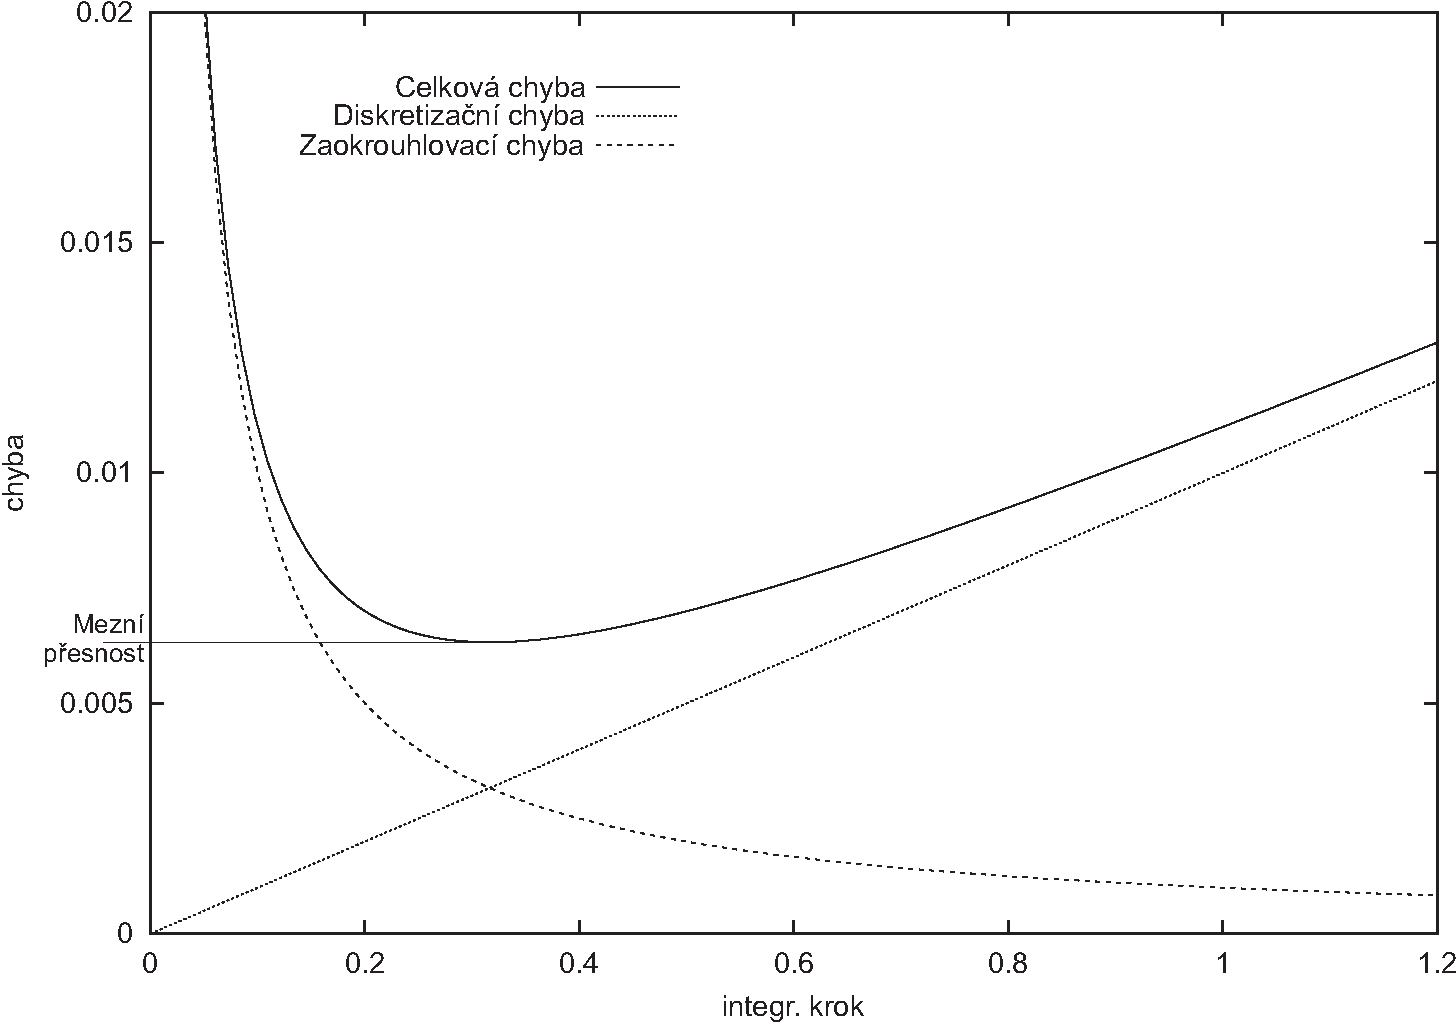
\includegraphics[width=0.98\textwidth]{chyby}\\
\caption[]{Vztah diskretizační, zaokrouhlovací a celkové chyby.}
\label{chyby}
\end{figure}
\subsubsection{Mezní přesnost metody}
V předešlých odstavcích jsme ukázali, že zkracováním integračního kroku můžeme
dosáhnout libovolného zmenšení diskretizační chyby Eulerovy metody. Zároveň 
ale zkracování kroku vede k růstu celkové zaokrouhlovací chyby. Celková chyba 
metody, která je součtem zmíněných dvou druhů chyb $e_i+r_i$ tak musí mít
pro nějakou hodnotu integračního kroku $h_0$ minimální hodnotu (viz Obr. \ref{chyby}). 
Této hodnotě říkáme {\em mezní přesnost} Eulerovy metody a zmenšení chyby pod tuto 
mez již nelze jinak, než užitím jiné metody, jejíž diskretizační chyba bude při
stejném integračním kroku menší. Zaokrouhlovací chyba je totiž do značné míry 
nezávislá na metodě a díky tomu lze zmenšením diskretizační chyby upravit mezní 
přesnost.

\subsection{Obecná jednokroková metoda}
Eulerova metoda popisovaná v minulé kapitole je speciálním případem obecné 
jednokrokové metody. Název {\em jednokroková metoda} označuje tu vlastnost metody,
že přibližná hodnota řešení $x_{i+1}$ v bodě $t_{i+1}$ je počítána pouze ze 
znalosti hodnoty přibližného řešení $x_i$ v bodě $t_i$.

Obecnou jednokrokovou metodu lze zapsat ve tvaru
\begin{equation}\label{1krmet}
\begin{array}{crl}
x_0 & =& \xi,\\
x_{i+1} &=&x_i+h \Phi(t_i,x_i,h),~~~~ i=0,\dots,n-1,
\end{array}
\end{equation}
přičemž funkce $\Phi$ musí mít nějaký vztah k pravé straně diferenciální rovnice $f$.

Definujme funkci $\bar\Phi(t,x,h)$ tak, aby při jejím dosazení do metody (\ref{1krmet}) 
za funkci $\Phi(t,x,h)$ vycházelo přesné řešení. Označíme-li $x(t)$ přesné řešení 
počáteční úlohy (\ref{pocul}), můžeme hledanou funkci $\bar\Phi$ zapsat takto:
\begin{equation}\label{delta}
\bar\Phi(t_i,x_i,h) = \left\{\begin{array}{ll}
\frac{x(t_{i+1})-x(t_i)}{h}&\mbox { pro }h>0,\\
f(t_i,x_i)&\mbox { pro }h=0.
\end{array}\right.
\end{equation}
Hodnota pro $h=0$ nemá praktický význam (metodu s nulovým integračním krokem nemá 
smysl budovat). Je dodefinována tak, aby funkce $\bar\Phi$ byla spojitá v okolí bodu 
$h=0$.

Bohužel, bez znalosti přesného řešení funkci $\bar\Phi$ nezískáme a bez znalosti funkce 
$\bar\Phi$ nespočítáme obecnou jednokrokovou metodou přesné řešení. Proto je třeba 
funkci $\Phi$ definovat jinak, než $\Phi\equiv\bar\Phi$. Je ale třeba ji hledat tak,
aby se pro malá $h$ funkce $\Phi$ nelišila od funkce $\bar\Phi$ příliš. Je patrné, že
nejjednodušší takovou volbou je právě Eulerova metoda s $\Phi(t,x,h)=f(t,x)$.

Volba $\Phi$ určuje přesnost obecné jednokrokové metody. Tu je možno kvantifikovat
veličinou, kterou nazveme {\em řád obecné jednokrokové metody}. Označme $\cal M$ 
podmnožinu množiny všech diferenciálních rovnic, jejichž pravé strany splňují 
předpoklady (\ref{predpokl}.i) a (\ref{predpokl}.ii). Řádem dané obecné jednokrokové 
metody na množině $\cal M$ pak označíme maximální přirozené číslo $p$, pro které
platí:
\begin{displaymath}
 L(x(t);h):=h[\Phi(t,x(t),h)-\bar\Phi(t,x(t),h)]=O(h^{p+1}),
\end{displaymath}
tj. je-li lokální chyba metody řádu $p+1$, je řád metody $p$.

Ve smyslu této definition má Eulerova metoda řád 1 na množině rovnic se spojitě 
diferencovatelnou pravou stranou. Na množině všech řešitelných rovnic její
řád nelze určit.

Předpokládejme, že funkce pravé strany $f$ má pro všechna $t\in\langle a,b\rangle$
všechny parciální derivace až do řádu $p$. Potom přesné řešení počáteční úlohy 
(\ref{pocul}) má derivace až do řádu $p+1$ a platí pro ně rovnice
\begin{eqnarray*}
\dot x &=& f(t,x)\\
\ddot x &=& \frac{\d}{\d t} f(t,x)=f_t(t,x) + f_x(t,x) f(t,x) =: \dot f(t,x)\\
x^{(3)} &=& \frac{\d^2}{\d t^2} f(t,x)=f_{tt}(t,x)+2 f_{tx}(t,x)f(t,x) + f_t(t,x)f_x(t,x) + \\ %\nonumber
&+&f_x^2(t,x)f(t,x) + f_{xx}(t,x)f^2(t,x) =: \ddot f(t,x)\\
x^{(4)} &=& \dots = f^{(3)}(t,x)\\
\vdots &&
\end{eqnarray*}
Zde indexy $_t$, resp. $_x$ značí parciální derivaci podle $t$, resp. $x$ a tečka 
značí totální derivaci podle $t$.

S předpokladem existence uvedených derivací tedy můžeme rozvinout přírůstek
$h\bar\Phi(t,x,h)$ v Taylorovu řadu v bodě $t$:
\begin{eqnarray*}
h\bar\Phi(t,x,h) &=& x(t+h) - x(t) = \\
&=&h\dot x(t) + \frac{h^2}{2!}\ddot x(t)+\dots+\frac{h^p}{p!}x^{(p)}(t)+O(h^{p+1})=\\
&=&hf(t,x)+ \frac{h^2}{2}\dot f(t,x)+\dots+\frac{h^p}{p!}f^{(p-1)}(t,x)+O(h^{p+1}),
\end{eqnarray*}
a tedy funkci $\bar\Phi$ můžeme psát ve tvaru
\begin{equation}\label{Taylor}
\bar\Phi(t,x,h) = f(t,x)+ \frac{1}{2}h\dot f(t,x)+\dots+\frac{1}{p!}h^{p-1}f^{(p-1)}(t,x)+O(h^{p}).
\end{equation}

Rovnice (\ref{Taylor}) nám nabízí přímo volit funkci $\Phi$ jako prvních $p$ členů
Taylorova rozvoje funkce $\bar\Phi$, tedy
\begin{displaymath}
\Phi(t,x,h) = f(t,x)+ \frac{1}{2}h\dot f(t,x)+\dots+\frac{1}{p!}h^{p-1}f^{(p-1)}(t,x).
\end{displaymath}
Tato metoda je označována termínem {\em metoda Taylorova rozvoje řádu $p$}, její řád
je $p$ na množině rovnic s $p$ krát spojitě diferencovatelnou pravou stranou. Ale
bohužel není příliš praktická. Pochybovači se mohou přesvědčit krátkým cvičením a 
pokusit se určit funkci $\Phi$ jako rozvoj do 3. řádu pro diferenciální rovnici 
$\dot x=x^2 + t^2$.

%%% 7. prednaska 2004:
\subsection{Runge-Kuttovy metody}
Závěr předchozí kapitoly nás přivedl k úloze sestrojit funkci $\Phi$ tak, aby se od
funkce $\bar\Phi$ lišila až ve členech řádu $h^p$, ale aby nebylo k jejímu sestrojení 
třeba hledat žádné derivace funkce $f$. Řešení takové úlohy je určeno skutečností,
že libovolnou derivaci každé funkce lze aproximovat lineární kombinací jejích hodnot 
ve vhodně zvolených bodech. Na této myšlence je založena celá třída jednokrokových 
metod nazývaných obecně {\em Runge-Kuttovy metody}.

Pro příklad si odvodíme třídu Runge-Kuttových metod řádu $p=2$.

Hledejme funkci $\Phi$ ve tvaru 
\begin{displaymath}
\Phi(t,x,h)=w_1k_1+w_2k_2,\mbox{ kde~} k_1=f(t,x), k_2=f(t+\alpha h,x+\beta h k_1),
\end{displaymath}
a $w_1$, $w_2$, $\alpha$ a $\beta$ jsou konstanty zvolené tak, aby rozvoj funkce 
$\Phi$ jako funkce proměnné $h$ byl shodný s rozvojem funkce $\bar\Phi$ do co 
největšího řádu.

Rozvojem funkce $\Phi$ v proměnné $h$ dostaneme
\begin{eqnarray*}
\Phi(t,x,h)\!&\!=\!&\! w_1 f(t,x)+ w_2 f(t+\alpha h,x+\beta h f(t,x))=w_1 f(t,x)+ \\
&\!+\!&\! w_2 f(t,x)+ w_2\alpha f_t(t,x) h+w_2\beta f_x(t,x)hf(t,x)+ O(h^2)=\\
&\!=\!&\! (w_1+w_2) f(t,x)+ w_2[\alpha f_t(t,x)+ \beta f_x(t,x)f(t,x)]h+O(h^2).
\end{eqnarray*}
Porovnáním členů rozvoje se vzorcem (\ref{Taylor}) dostaneme pro konstanty
$w_1$, $w_2$, $\alpha$ a $\beta$ soustavu tří rovnic
\begin{displaymath}
w_1+w_2=1,~~~~w_2 \alpha=\frac 12,~~~~w_2\beta=\frac 12.
\end{displaymath}
Ta má nekonečně mnoho řešení, která je možno zapsat v parametrickém tvaru
\begin{equation}\label{RKmet2r}
w_1=1-s,~~~~w_2=s,~~~~\alpha=\beta=\frac 1{2s},
\end{equation}
kde parametr $s$ je libovolné nenulové reálné číslo.

Žádnou volbou parametrů $w_1$, $w_2$, $\alpha$ a $\beta$ nelze docílit shody
rozvoje funkcí $\Phi$ a $\bar\Phi$ až do třetího řádu. Našli jsme tedy celou 
sadu metod řádu 2 na množině rovnic s třikrát spojitě diferencovatelnou funkcí 
pravé strany. Pro její sestrojení nepotřebujeme počítat derivace pravé strany,
namísto toho je třeba však pro výpočet jednoho integračního kroku počítat 
dvakrát hodnoty funkce $f$ ve dvou různých bodech.

Z právě odvozené třídy metod jsou prakticky užívány dvě. Dosazením parametru 
$s=1$ do (\ref{RKmet2r}) dostaneme tzv. {\em modifikovanou Eulerovu metodu}
\begin{equation}\label{modifEuler}
x_{i+1}=x_i + h f(t_i+\frac 12 h, x_i+\frac 12 hf(t_i,x_i)),
\end{equation}
kterou lze geometricky názorněji přepsat do tvaru
\begin{eqnarray*}
x_{i+1}&=&x_i + h k_2, \mbox{~kde}\\
k_1 &=& f(t_i,x_i),\\
k_2 &=& f(t_i+\frac 12 h, x_i+\frac 12 h k_1).
\end{eqnarray*}
Dosadíme-li do (\ref{RKmet2r}) za $s=1/2$, definujeme tzv. {\em Heunovu metodu}
\begin{equation}\label{Heun}
x_{i+1}=x_i + \frac 12h[f(t_i,x_i)+f(t_i+h, x_i+hf(t_i,x_i))],
\end{equation}
kterou podobně přepíšeme ve tvaru
\begin{eqnarray*}
x_{i+1}&=&x_i + \frac 12 h (k_1 + k_2), \mbox{~kde}\\
k_1 &=& f(t_i,x_i),\\
k_2 &=& f(t_i+h, x_i+h k_1).
\end{eqnarray*}


Vyjádříme-li podstatu Eulerovy metody slovy tak, že přírůstek odhadu řešení 
v $i$-tém časovém kroku je dán hodnotou funkce $f$ v bodě $(t_i,x_i)$, pak 
lze obě uvedené metody geometricky interpretovat tak, že přírůstek odhadu
řešení je v $i$-tém časovém kroku dán v odhadem hodnoty funkce $f$ mezi body
$(t_i,x_i)$ a $(t_{i+1}, x_{i+1})$. V případě modifikované Eulerovy metody je
odhadnut střední bod úsečky $\overline{(t_i,x_i),(t_{i+1}, x_{i+1})}$ a v něm
je vyčíslena hodnota funkce $f$. V případě Heunovy metody je uvažován 
algebraický průměr hodnot $f(t_i,x_i)$ a $f(t_{i+1}^*, x_{i+1}^*)$, kde
bod $(t_{i+1}^*, x_{i+1}^*)$ je odhadem bodu $(t_{i+1}, x_{i+1})$ Eulerovou
metodou.

\subsubsection{Obecná Runge-Kuttova metoda}
Obecná Runge-Kuttova metoda má funkci $\Phi$ předepsanou ve tvaru:
\begin{eqnarray*}
\Phi(t,x,h) &=& \sum_{j=1}^s w_jk_j,\mbox{~kde}\\
k_1 &=& f(t,x),\\
k_j &=& f\left(t+\alpha_j h, x+h\sum_{l=1}^{j-1}\beta_{jl}k_l\right), j=2,\dots,s.
\end{eqnarray*}
K výpočtu funkce $\Phi$ je tak třeba vypočítat $s$-krát hodnotu pravé strany $f$.

Lze ukázat, že parametry v každé Runge-Kuttově metodě lze volit tak, že pro její 
řád $p=p(s)$ platí $\lim_{s\to\infty} p = \infty$. Pro $s\leq 4$ je možno na 
množině diferenciálních rovnic s dostatečně hladkými pravými stranami docílit
řádu $p(s)=s$, pro $s>4$ roste funkce $p(s)$ pomaleji než $s$. Z tohoto důvodu
a také proto, že soustavy nelineárních rovnic svazujících koeficienty $w_j$, 
$\alpha_j$ a $\beta_{jl}$ jsou pro $s>4$ velmi složité, se prakticky 
Runge-Kuttových metod řádu většího než 4 užívá velmi zřídka.
Pro příklad složitosti nelineárních soustav rovnic svazujících koeficienty 
uvádíme případ, kdy $s=4$:
\begin{eqnarray*}
\alpha_2 &=& \beta_{21},\\
\alpha_3 &=& \beta_{31}+\beta_{32},\\
\alpha_4 &=& \beta_{41}+\beta_{42}+\beta_{43},\\
w_1+w_2+w_3+w_4 &=& 1,\\
w_2\alpha_2+w_3\alpha_3+w_4\alpha_4 &=& \frac 12,\\
w_2\alpha_2^2+w_3\alpha_3^2+w_4\alpha_4^2 &=& \frac 13,\\
w_2\alpha_2^3+w_3\alpha_3^3+w_4\alpha_4^3 &=& \frac 14,\\
w_3\alpha_2\beta_{32}+w_4(\alpha_2\beta_{42}+\alpha_3\beta_{43})&=& \frac 16,\\
w_3\alpha_2^2\beta_{32}+w_4(\alpha_2^2\beta_{42}+\alpha_3^2\beta_{43})&=& \frac 1{12},\\
w_3\alpha_2\alpha_3\beta_{32}+w_4(\alpha_2\beta_{42}+\alpha_3\beta_{43})\alpha_4&=& \frac 18,\\
w_4\alpha_2\beta_{32}\beta_{43}&=& \frac 1{24}.
\end{eqnarray*}

Uveďme několik často užívaných Runge-Kuttových metod. Jedna z metod třetího 
řádu nese rovněž jméno {\em Heunova metoda} a má tvar
\begin{eqnarray*}
x_{i+1} &=& x_i+ \frac 14 h (k_1+3k_3)\\
k_1 &=& f(t_i,x_i),\\
k_2 &=& f(t_i+\frac 13 h,x_i+\frac 13 hk_1),\\
k_3 &=& f(t_i+\frac 23 h,x_i+\frac 23 hk_2).
\end{eqnarray*}

Tzv. {\em standardní Runge-Kuttova metoda} je čtvrtého řádu:
\begin{eqnarray*}
x_{i+1} &=& x_i+ \frac 16 h (k_1+2k_2+2k_3+k_4)\\
k_1 &=& f(t_i,x_i),\\
k_2 &=& f(t_i+\frac 12 h,x_i+\frac 12 hk_1),\\
k_3 &=& f(t_i+\frac 12 h,x_i+\frac 12 hk_2),\\
k_4 &=& f(t_i+h,x_i+hk_3).
\end{eqnarray*}

Další často užívanou metodou čtvrtého řádu je tzv. {\em tříosminové pravidlo}:
\begin{eqnarray*}
x_{i+1} &=& x_i+ \frac 18 h (k_1+3k_2+3k_3+k_4)\\
k_1 &=& f(t_i,x_i),\\
k_2 &=& f(t_i+\frac 13 h,x_i+\frac 13 hk_1),\\
k_3 &=& f(t_i+\frac 23 h,x_i-\frac 13 hk_1+hk_2),\\
k_4 &=& f(t_i+h,x_i+hk_1-hk_2+hk_3).
\end{eqnarray*}

Metody vyšších řádů nejsou, jak už jsme uvedli, užívány často. Jejich odvození 
i implementace jsou sice složitější, k jejich realizaci je třeba více početních 
operací na jeden integrační krok, avšak jsou přesnější a proto není třeba pro 
stejnou přesnost tak krátký časový krok jako při užití metod nižších řádů, což
může jejich nevýhody kompenzovat i převážit.

Populární metodou pátého řádu je {\em Fehlbergova metoda}:
\begin{eqnarray*}
x_{i+1} &=& x_i+ h\left(\frac {16}{135} k_1+\frac {6656}{12825} k_3+\frac {28561}{56430} k_4+\frac 9{50} k_5+\frac 2{55} k_6\right)\\
k_1 &=& f(t_i,x_i),\\
k_2 &=& f(t_i+\frac 14 h,x_i+\frac 14 hk_1),\\
k_3 &=& f(t_i+\frac 38 h,x_i+\frac 1{32} h(3k_1+9k_2)),\\
k_4 &=& f(t_i+\frac {12}{13}h,x_i+\frac 1{2197}h(1932k_1-7200k_2+7296k_3)),\\
k_5 &=& f(t_i+h,x_i+h(\frac{439}{216}k_1-8k_2+\frac{3680}{513}k_3-\frac{845}{4104}k_4)),\\
k_6 &=& f(t_i+\frac 12 h,x_i+h(-\frac 8{27}k_1+2k_2-\frac{3544}{2565}k_3+\frac{1859}{4104}k_4-\frac{11}{40}k_5)).
\end{eqnarray*}

Z metod šestého řádu uvádíme {\em Huťovu metodu}:
\begin{eqnarray*}
x_{i+1} &=& x_i+ \frac 1{840}h\left(41k_1+216k_3+27k_4+272k_5+27k_6+216k_7+41k_8\right)\\
k_1 &=& f(t_i,x_i),\\
k_2 &=& f(t_i+\frac 19 h,x_i+\frac 19 hk_1),\\
k_3 &=& f(t_i+\frac 16 h,x_i+\frac 1{24} h(k_1+3k_2)),\\
k_4 &=& f(t_i+\frac 13 h,x_i+\frac 16 h(k_1-3k_2+4k_3)),\\
k_5 &=& f(t_i+\frac 12 h,x_i+\frac 18 h(-5k_1+27k_2-24k_3+6k_4)),\\
k_6 &=& f(t_i+\frac 23 h,x_i+\frac 19 h(221k_1-981k_2+867k_3-102k_4+k_5)),\\
k_7 &=& f(t_i+\frac 56 h,x_i+\frac 1{48} h(-183k_1+678k_2-472k_3-66k_4+80k_5+3k_6)),\\
k_8 &=& f(t_i+h,x_i+\frac 1{82}h(716k_1-2079k_2+1002k_3+834k_4-454k_5-9k_6+72k_7)).
\end{eqnarray*}

\subsubsection{Chyby Runge-Kuttových metod}

Pro diskretizační chybu Runge-Kuttových metod lze dokázat větu:
\begin{theorem}\label{Veta3.2}
Buď dána Runge-Kuttova metoda řádu $p$ na množině rovnic s $p+1$ krát spojitě 
diferencovatelnou pravou stranou a počáteční úloha z této množiny. Označíme-li
$x(t)$ přesné řešení úlohy a $x_i$ jeho aproximaci získanou danou metodou, 
existují konstanty $M$ a $h_0$ nezávislé na zvolené úloze takové, že pro každé 
$h<h_0$ platí:
\begin{equation}\label{odhadRK}
|x_i-x(t_i)| \leq M h^p E_L(t_i-a), i=0,\dots,n,
\end{equation}
kde funkce $E_L(t)$ je definována v tvrzení věty \ref{Veta2.2} na straně
\pageref{Veta2.2}.
\end{theorem}

Neznáme-li velikost konstanty $M$ (což je velmi častý případ), vyplývá z věty 
\ref{Veta3.2} pouze rychlost konvergence Runge-Kuttových metod. Není tedy nijak 
užitečná k odhadu chyby. Všimněme si ale, že ve srovnání s Eulerovou metodou (viz
větu \ref{Veta2.2}) klesá chyba při klesajícím $h$ rychleji (zde klesá s $h^p$,
u Eulerovy metody s $h$).

%\begin{theorem}\label{Veta3.3}
%Nechť jsou splněny předpoklady věty \ref{Veta3.2} a nechť je $\tilde y_i$ 
%aproximace řešení počáteční úlohy Runge-Kuttovou metodou poškozenou 
%numerickou chybou ve tvaru:
%\begin{equation}\label{poskRK}
%\begin{array}{crl}
%\tilde y_0 & =& \eta,\\
%\tilde y_{i+1} &=&\tilde y_i+h[\Phi(x_i,\tilde y_i,h) + h^q\Theta_i K],~~~~ i=0,\dots,n-1,
%\end{array}
%\end{equation}
%kde $K$ je konstanta a $\Theta_i$ je posloupnost omezená číslem 1, tj. $|\Theta_i|\leq 1$.
%Potom existuje $h_0$ a $M_1$ tak, že pro $h<h_0$ a $i=0,\dots,n$ platí
%\begin{equation}
%|\tilde y_i-y(x_i)| \leq M_1 h^r E_L(x_i-a),
%\end{equation}
%kde $r=\min(p,q)$.
%\end{theorem}

%%% 8. prednaska 2004:
Pro odhad velikosti chyby je užitečný asymptotický odhad chyby, který vyjadřuje
následující věta:
\begin{theorem}\label{Veta3.4}
Nechť jsou splněny předpoklady (\ref{predpokl}.i) a (\ref{predpokl}.ii) a nechť
je $x_i$ přibližné řešení úlohy vypočtené Runge-Kuttovou metodou řádu $p\geq 1$.
Nechť navíc mají pravá strana $f$ a funkce Runge-Kuttovy metody $\Phi$ $p+1$ 
spojitých parciální derivace podle všech proměnných v oblasti 
$\langle a,b\rangle\times R$, resp. 
$\langle a,b\rangle\times R\times\langle 0,h_0\rangle$.
Pak lze celkovou diskretizační chybu přibližného řešení vypočteného danou 
Runge-Kuttovou metodou zapsat ve tvaru
\begin{equation}\label{asympRK}
x_i-x(t_i)=e(t_i)h^p+O(h^{p+1}),
\end{equation}
kde je funkce $e(t)$ řešením diferenciální rovnice
\begin{displaymath}
\dot e=\frac{\partial}{\partial x}f(t,x(t))e-\varphi(t,x(t))
\end{displaymath}
s počáteční podmínkou $e(a)=0$, přičemž
\begin{eqnarray*}
\varphi(t,x)&=&\left.\frac 1{p!}\frac{\partial^p}{\partial h^p}\left[\bar\Phi(t,x,h)-\Phi(t,x,h)\right]\right|_{h=0}=\\
&=&\frac 1{(p+1)!}f^{(p)}(t,x)-\left.\frac 1{p!}\frac{\partial^p\Phi(t,x,h)}{\partial h^p}\right|_{h=0}
\end{eqnarray*}
\end{theorem}

Z věty \ref{Veta3.4} vyplývá {\em aposteriorní odhad} chyby metodou polovičního 
kroku analogický k (\ref{polkrok}):
\begin{equation}\label{polkrokRK}
x(t;h)-x(t)=\frac {2^p}{2^p-1}[x(t;h)-x(t;\frac h2)]+O(h^{p+1}).
\end{equation}

\begin{figure}[ht]
\centering
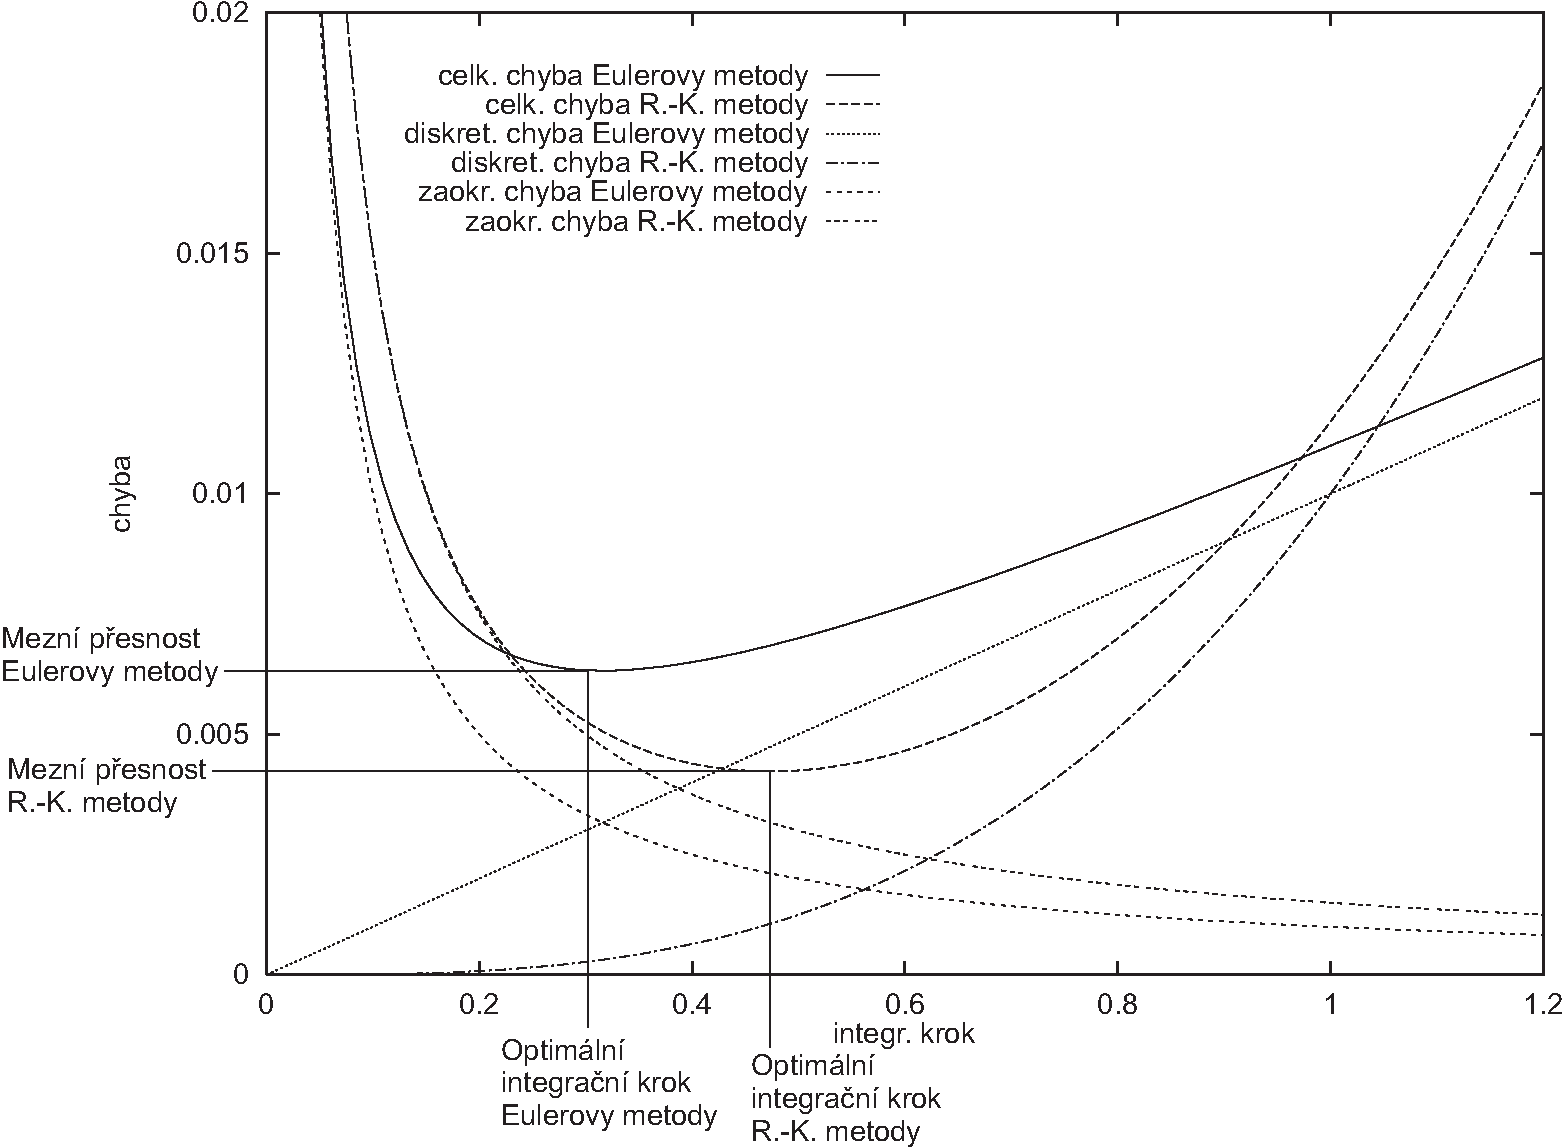
\includegraphics[width=0.98\textwidth]{chyby3}\\
\caption[]{Porovnání mezní přesnosti Eulerovy a Runge-Kuttovy metody.}
\label{chyby1}
\end{figure}

%%% tohle bylo v 7. prednasce 2004:
Zavedeme-li lokální zaokrouhlovací chybu podobně jako pro Eulerovu metodu vztahy
\begin{equation}\label{poskRK}
\begin{array}{crl}
\tilde x_0 & =& \xi,\\
\tilde x_{i+1} &=&\tilde x_i+h \Phi(t_i,\tilde x_i,h) + \varepsilon_i,~~~~ i=0,\dots,n-1,
\end{array}
\end{equation}
lze pro velikost celkové zaokrouhlovací chyby dokázat následující větu:
\begin{theorem}\label{Veta3.5}
Nechť pravá strana $f$ splňuje předpoklady (\ref{predpokl}.i) a (\ref{predpokl}.ii) 
a $\Phi$ je funkce Runge-Kuttovy metody. Nechť je lokální zaokrouhlovací chyba 
$\varepsilon_i$ omezená konstantou $\varepsilon$. Pak pro celkovou zaokrouhlovací 
chybu platí
\begin{equation}\label{zaokrchRK}
|\tilde x_i-x_i|\leq \frac\varepsilon h E_L(t_i-a), i=0,\dots,n-1.
\end{equation}
\end{theorem}

Tvrzení věty \ref{Veta3.5} je v podstatě totožné s tvrzením věty \ref{Veta2.5}.
Zaokrouhlovací chyba se tedy projevuje stejně u Eulerovy metody, jako Runge-Kuttových 
metod libovolného řádu. Důsledkem této skutečnosti a větší rychlosti konvergence 
diskretizační chyby Runge-Kuttových metod vyšších řádů je skutečnost, že mezní 
přesnost Runge-Kuttových metod je lepší než mezní přesnost Eulerovy metody a je
dosahována při větším integračním kroku. Právě vyslovené tvrzení je ilustrováno na
obrázku \ref{chyby1}. Pochopitelně podobný vztah platí i mezi dvěma Runge-Kuttovými 
metodami různých řádů.
%%% az sem to bylo v 7. prednasce 2004

\section[Numerické řešení ODR s okrajovými podmínkami]{Numerické řešení obyčejných 
diferenciálních rovnic s~okrajovými podmínkami}

{\em Dvoubodovou okrajovou úlohou}, nebo stručně {\em okrajovou úlohou} pro 
soustavu obyčejných diferenciálních rovnic prvního řádu
\begin{equation}\label{SLODR2}
\dot {\vc x}=\vc f(t,\vc x),
\end{equation}
kde $\vc x=\left(\begin{array}{c}x_1\\ \vdots\\x_m\end{array}\right)$ a 
$\vc f=\left(\begin{array}{c}f_1\\ \vdots\\f_m\end{array}\right)$,
rozumíme úlohu najít takové řešení soustavy (\ref{SLODR2}), které
splňuje {\em okrajové podmínky}
\begin{equation}\label{okp}
\vc r(\vc x(a),\vc x(b))=\vc 0,
\end{equation}
kde $\vc r$ je $m$-složková vektorová funkce $2m$ proměnných a navzájem různé 
body $a$ a $b$ leží v intervalu, v němž hledáme řešení. Nejčastěji právě jeho
krajní body -- odtud název \uv{okrajové podmínky}.

Je-li možné okrajové podmínky přepsat ve tvaru
\begin{equation}\label{sepokp}
\begin{array}{rcl}
\vc r_1(\vc x(a))&=&\vc 0,\\
\vc r_2(\vc x(b))&=&\vc 0,
\end{array}
\end{equation}
kde $r_1$, resp. $r_2$ jsou $m_1$-, resp. $m_2$-složkové vektorové funkce $m$
proměnných, přičemž $m_1+m_2=m$, říkáme, že jde o {\em separované okrajové 
podmínky}.

Jiným speciálním případem jsou {\em lineární okrajové podmínky} ve tvaru
\begin{equation}\label{linokp}
{\tn U}\vc x(a)+ {\tn V}\vc x(b)=\vc c,
\end{equation}
kde $\tn U$ a $\tn V$ jsou čtvercové matice řádu $m$ a $\vc c$ je $m$-rozměrný
vektor. {\em Lineární separované okrajové podmínky} pak mají tvar
\begin{equation}\label{linsepokp}
\begin{array}{rcl}
{\tn V}_1 \vc x(a)&=&\vc v_1,\\
{\tn V}_2 \vc x(b)&=&\vc v_2,
\end{array}
\end{equation}
kde ${\tn V}_1$, resp. ${\tn V}_2$ jsou obdélníkové matice typu $m_1\times m$, 
resp. $m_2\times m$ a $\vc v_1$, resp. $\vc v_2$ vektory o $m_1$, resp. $m_2$
složkách (zase $m_1+m_2=m$).

Podobně, jako jsme zavedli počáteční úlohu pro obyčejnou diferenciální rovnici 
vyššího řádu (viz rovnice (\ref{LODRm}) a další), můžeme zavést i okrajovou 
úlohu pro takovou rovnici.

Všimněme si rovněž, že položíme-li v rovnici (\ref{linokp}) pro lineární 
okrajové podmínky za $\tn U$ jednotkovou matici $\tn E$ a za $\tn V$ nulovou
matici $\tn O$, dostaneme předpis pro počáteční podmínky.
Počáteční úloha je tedy velmi speciálním případem okrajové úlohy. A bohužel,
zatímco stačí splnit předpoklady (\ref{predpokl}), aby existovalo jednoznačné 
řešení počáteční úlohy, žádné podobně jednoduché tvrzení pro okrajové úlohy
nelze najít. U sebejednodušší diferenciální rovnice můžeme okrajové podmínky
předepsat tak, že řešení buď vůbec neexistuje, anebo jich existuje víc.
Pro příklad uvedeme diferenciální rovnici druhého řádu 
\begin{equation}\label{example}
\ddot x + x = 0,
\end{equation}
kterou lze ekvivalentně převést na soustavu dvou rovnic prvního řádu
\begin{displaymath}
\begin{array}{rcl}
\dot x_1&=&x_2,\\
\dot x_2&=&-x_1.
\end{array}
\end{displaymath}
Každé její řešení lze zapsat ve tvaru
\begin{displaymath}
x(t) = C_1 \cos t + C_2 \sin t,
\end{displaymath}
kde $C_1$ a $C_2$ jsou libovolné konstanty.
Zvolíme-li okrajové podmínky
\begin{equation}\label{OKP1}
x(0) = 0, ~~~~~~ x(\pi)=0,
\end{equation}
je řešením okrajové úlohy (\ref{example}), (\ref{OKP1}) nekonečně mnoho funkcí
ve tvaru $C \sin t$, kde $C$ je libovolné číslo. Naopak, s okrajovými podmínkami
\begin{equation}\label{OKP2}
x(0) = 0, ~~~~~~ x(\pi)=1,
\end{equation}
nemá rovnice (\ref{example}) žádné řešení.

\subsection{Metoda střelby}
Je jednou z metod řešení okrajových úloh založených na převodu úlohy 
s okrajovými podmínkami na ekvivalentní počáteční úlohu. Její princip 
budeme ilustrovat na konkrétní úloze.

\subsubsection{Lineární samoadjungovaná diferenciální rovnice}
Uvažujme lineární samoadjungovanou diferenciální rovnici druhého řádu
\begin{equation}\label{samoadj}
-(p(t)\dot x)\dot{}+q(t)x=f(t)
\end{equation}
s {\em Dirichletovými okrajovými podmínkami}
\begin{equation}\label{dirokp}
x(a) = \gamma_1,~~~~~~ x(b)=\gamma_2.
\end{equation}
Předpokládejme, že funkce $p$, $\dot p$, $q$ a $f$ jsou spojité v intervalu 
$\langle a,b\rangle$, že existuje kladná konstanta $p_0$ taková, že
\begin{displaymath}
p(t)\geq p_0, ~~~ t\in\langle a,b\rangle,
\end{displaymath}
a že je 
\begin{displaymath}
q(t)\geq 0, ~~~ t\in\langle a,b\rangle.
\end{displaymath}
Lze dokázat, že za těchto podmínek je okrajová úloha (\ref{samoadj}), 
(\ref{dirokp}) jednoznačně řešitelná.

Zadaná rovnice rovněž splňuje předpoklady (\ref{predpokl}). Proto pro
každou počáteční podmínku
\begin{equation}\label{pocpmetstr}
x(a) = \gamma_1,~~~~~~ \dot x(a)=\alpha,
\end{equation}
kde $\alpha$ je libovolné číslo, existuje právě jedna funkce $y(x)$ 
řešící počáteční úlohu (\ref{samoadj}), (\ref{pocpmetstr}). Označme 
řešení takové úlohy $x(t;\alpha)$.

Řešení $x(t;\alpha)$ splňuje diferenciální rovnici (\ref{samoadj})
a jednu z okrajových podmínek (\ref{dirokp}) a závisí na parametru 
$\alpha$. Nalezneme-li tedy takovou hodnotu $\alpha^*$ parametru
$\alpha$, pro kterou bude platit druhá okrajová podmínka, tj. 
\begin{equation}\label{okpmetstr}
x(b;\alpha^*) = \gamma_2,
\end{equation}
dostaneme řešení okrajové úlohy (\ref{samoadj}), (\ref{dirokp}).
Převedli jsme tak původní okrajovou úlohu na úlohu nalezení 
počáteční podmínky odpovídající zadaným okrajovým podmínkám a řešení
tak vzniklé počáteční úlohy. Nyní je patrné, proč se tato metoda nazývá
metodou střelby.

K nalezení hledané hodnoty $\alpha^*$ je třeba znát základy teorie 
lineárních diferenciálních rovnic, kterou čtenář v potřebném rozsahu najde
například v \cite{Nagy}. Zde uvedeme a použijeme pouze její závěry.

Označíme-li $z(x)$ řešení homogenní rovnice příslušné k (\ref{samoadj}), tj.
\begin{displaymath}
-(p(t)\dot z)\dot{}+q(t)z=0
\end{displaymath}
s počátečními podmínkami
\begin{displaymath}
z(a) = 0,~~~~~~ \dot z(a)=1,
\end{displaymath}
pak pro libovolné $\alpha$ platí:
\begin{displaymath}
x(t;\alpha) = x(t;0)+\alpha z(t)
\end{displaymath}
a speciálně pro $t=b$ je $x(b;\alpha) = x(b;0)+\alpha z(b)$. Řešení rovnice
(\ref{okpmetstr}) má tedy tvar
\begin{equation}\label{alfa*}
\alpha^*=\frac{\gamma_2-x(b;0)}{z(b)}.
\end{equation}
Pochopitelně za předpokladu, že $z(b)\neq 0$, což je zajištěno předpoklady, které 
jsme kladli na funkce $p$, $q$ a $f$.

Řešení lineární okrajové úlohy (\ref{samoadj}), (\ref{dirokp}) metodou střelby 
spočívá tedy ve dvojím řešení počáteční úlohy (pro $x(t;0)$ a $z(t)$) a v lineárním
zkombinování uvedených řešení podle vzorce
\begin{displaymath}
x(t;\alpha^*) = x(t;0)+\alpha^* z(t),
\end{displaymath}
kde $\alpha^*$ spočteme z rovnice (\ref{alfa*}).

\subsubsection*{Příklad}
Pro ilustraci uvedeme příklad řešení konkrétní úlohy uvedenou metodou. 
Řešme rovnici
\begin{equation}\label{priklmetstr}
-\ddot x + 100 x = 0
\end{equation}
s lineárními separovanými okrajovými podmínkami
\begin{equation}\label{priklOKP1}
x(0)=1, ~~~~~~ x(0{,}1)=1.
\end{equation}
Podotkněme, že tuto úlohu umíme řešit analyticky. Její řešení má tvar
\begin{equation}\label{reseniprikl2}
x(t)=
\frac 1{e+1} e^{10t}+\frac e{e+1} e^{-10t}.
\end{equation}

Pro její řešení metodou střelby použijeme vzorec (\ref{alfa*}), přičemž
\begin{eqnarray*}
x(t;0)&=&\frac 12 e^{10t}+\frac 12 e^{-10t},\\
z(t)&=&\frac 1{20}e^{10t}-\frac 1{20}e^{-10t}
\end{eqnarray*}
a tedy (při $b=0{,}1$)
\begin{eqnarray*}
\alpha^*&=&\frac{1-\frac 12 e-\frac 12 e^{-1}}{\frac 1{20}e-\frac 1{20}e^{-1}}
=10\frac{2e-e^2-1}{e^2-1}=-10\frac{(e-1)^2}{(e-1)(e+1)}=\\
 &=& 10\frac{1-e}{e+1}\doteq-4{,}6211715726.
\end{eqnarray*}
Počítáme-li s přesností na šest platných míst, počítač určí hodnotu
$\alpha^*$ na $-4{,}62117$ a přibližné řešení na:
\begin{eqnarray*}
x(t;-4{,}62117)&=&x(t;0)-4{,}62117 z(t) = \\
&=&\frac 12 e^{10t}+\frac 12 e^{-10t}-0{,}462117(\frac 12 e^{10t}-\frac 12 e^{-10t})\doteq\\
&\doteq& 0{,}268942 e^{10t} + 0{,}731059 e^{-10t}
\end{eqnarray*}
a pravá okrajová podmínka bude přibližně splněna:
\begin{eqnarray*}
x(0{,}1;-4{,}62117)&\doteq& 0{,}268942 e + 0{,}731059 e^{-1}
\doteq 1{,}000002.
\end{eqnarray*}

%%% 9. prednaska 2004:
\subsubsection{Soustava lineárních diferenciálních rovnic}
Nyní řešme soustavu lineárních diferenciálních rovnic
\begin{equation}\label{SLODR}
\dot{\vc x}={\tn A}(t)\vc x+\vc b(t)
\end{equation}
s lineárními okrajovými podmínkami (\ref{linokp}). Zde je $\tn A$ čtvercová
matice řádu $m$, jejímiž prvky jsou spojité funkce a $\vc b$ je $m$-rozměrný
vektor spojitých funkcí. Tentokrát označíme $\vc x(t;\vc\alpha)$ řešení rovnice 
(\ref{SLODR}) s počátečními podmínkami
\begin{displaymath}
\vc x(a)=\vc\alpha
\end{displaymath}
a 
\begin{displaymath}
\vc F(\vc\alpha):=r(\vc\alpha,x(b;\vc\alpha))={\tn U}\vc\alpha+{\tn V}\vc x(b;\vc\alpha)-\vc c.
\end{displaymath}
Úloha tentokrát zní: najít takovou hodnotu $\vc\alpha^*$ neznámé $\vc\alpha$, že bude platit
rovnost
\begin{equation}\label{linokpmetstr}
\vc F(\vc\alpha^*)=0.
\end{equation}

Řešení počáteční úlohy pro soustavu lineárních rovnic $\vc x(t;\vc\alpha)$ (viz 
\cite{Nagy}) lze psát ve tvaru
\begin{displaymath}
\vc x(t;\vc\alpha)={\cal U}(t)\vc\alpha+\vc x(t;0),
\end{displaymath}
kde $\cal U$ je standardní fundamentální matice řešení soustavy 
(\ref{SLODR}) v bodě $a$, jejíž $i$-tý sloupec je řešením homogenní diferenciální 
rovnice
\begin{equation}\label{DRproSFM}
\dot {\vc x}={\tn A}(t)\vc x
\end{equation}
s počátečními podmínkami
\begin{equation}\label{OKPproSFM}
x_i(a)=1, ~~~~ x_j(a)=0, ~j\neq i.
\end{equation}
Speciálně pro bod $b$ platí $\vc x(b;\vc\alpha)={\cal U}(b)\vc\alpha+\vc x(b;0)$ a po
dosazení do rovnice (\ref{linokpmetstr}) dostáváme pro $\vc\alpha^*$ vztah
\begin{equation}\label{linalfa*}
\vc\alpha^* = [{\tn U}+{\tn V}{\cal U}(b)]^{-1}[\vc c-{\tn V}\vc x(b;0)],
\end{equation}
samozřejmě za podmínky, že uvedená inverzní matice existuje.

K řešení okrajové úlohy (\ref{SLODR}), (\ref{linokp}) metodou střelby je tedy
třeba provést $m$ řešení úloh s počátečními podmínkami pro získání matice $\cal U$,
jedno další řešení úlohy s počátečními podmínkami pro získání funkce $\vc x(t;\vc 0)$,
vyřešit jednu soustavu lineárních algebraických rovnic (\ref{linalfa*}) a potom
spočítat lineární kombinaci podle vzorce
\begin{equation}\label{linreseni}
\vc x(t;\vc\alpha^*) = {\cal U}(t)\vc\alpha^*+\vc x(t;\vc 0).
\end{equation}

\subsubsection{Obtíže metody střelby}
Tato kapitola bude věnována jednomu zdánlivě jednoduchému konkrétnímu příkladu: 
řešme znovu rovnici (\ref{priklmetstr})
\begin{displaymath}
-\ddot x + 100 x = 0
\end{displaymath}
s jinými lineárními separovanými okrajovými podmínkami
\begin{equation}\label{priklOKP2}
x(0)=1, ~~~~~~ x(10)=1.
\end{equation}
Její analytické řešení má tvar
\begin{equation}\label{reseniprikl1}
x(t)=\frac 1{e^{100}-e^{-100}} \left[(1-e^{-100}) e^{10t}+(e^{100}-1) e^{-10t}\right].
\end{equation}

Pro její řešení metodou střelby použijeme znovu vzorec (\ref{alfa*}), přičemž je, 
podobně jako v příkladě úspěšné aplikace metody střelby,
\begin{eqnarray*}
x(t;0)&=&\frac 12 e^{10t}+\frac 12 e^{-10t},\\
z(t)&=&\frac 1{20}e^{10t}-\frac 1{20}e^{-10t}
\end{eqnarray*}
a tedy (při $b=10$)
\begin{displaymath}
\alpha^*=-10+ 20\frac{1-e^{-100}}{e^{100}-e^{-100}}.
\end{displaymath}
Počítáme-li s přesností na několik desetiných míst, počítač určí hodnotu
$\alpha^*$ na $-10$. V takovém případě nebude druhá okrajová podmínka splněna
ani přibližně (je totiž $y(10;-10)=e^{-100}$).

Tento výsledek je způsoben tím, že uvedená úloha je citlivá na počáteční 
podmínku -- malá změna počáteční podmínky způsobí velkou změnu hodnoty
funkce v koncovém bodě. Koncový bod je zkrátka příliš daleko od počátečního 
bodu intervalu, ve kterém hledáme řešení. Problémy tohoto typu lze řešit 
malou úpravou metody, která dostala název {\em metoda střelby na více cílů}. 
Jí je věnována následující kapitola.

\subsection{Metoda střelby na více cílů}
Problém úlohy (\ref{priklmetstr}), (\ref{priklOKP2}) byl způsoben tím, že 
interval, na němž jsme 
ji řešili byl tak dlouhý, že se stala pravá okrajová podmínka \uv{přecitlivělou}
na volbu počáteční podmínky náhradní počáteční úlohy. Tomuto problému lze předejít 
prostě tím, že interval, na němž úlohu řešíme, zkrátíme. Pochopitelně, máme-li
předepsané okrajové podmínky v bodech $a$ a $b$, nelze zkrátit interval mezi nimi.
Lze ho však rozdělit na několik kratších intervalů a tím problému naznačenému 
v minulé kapitole předejít.

Buď dána okrajová úloha (\ref{SLODR2}), (\ref{okp}) a zvolme v intervalu 
$\langle a,b\rangle$ body $t_1$, \dots, $t_{n-1}$ tak, že $t_0=a<t_1<\dots<t_{n-1}<b=t_n$.
Zaveďme si ještě přesnější značení $\vc x(t;t_k,\vc\alpha_k)$ pro řešení rovnice
(\ref{SLODR2}) s počáteční podmínkou
\begin{displaymath}
\vc x(t_k)=\vc\alpha_k=(\alpha_{k,1},\dots,\alpha_{k,m})^T.
\end{displaymath}

Naším úkolem bude najít $n+1$ vektorů $\vc\alpha_0,\dots,\vc\alpha_n$ tak, aby 
platilo
\begin{equation}\label{metstrnvc1}
\vc x(t_{k+1};t_k,\vc\alpha_k)=\vc\alpha_{k+1}, ~~~~ k=0,\dots,n-1,
\end{equation}
a zároveň aby byla splněna okrajová podmínka (\ref{okp}), tj.
\begin{equation}\label{metstrnvc2}
\vc r(\vc\alpha_0,\vc\alpha_n)=0.
\end{equation}
Potom bude hledané řešení okrajové úlohy (\ref{SLODR2}), (\ref{okp}) popsáno
funkcí
\begin{equation}\label{metstrnvc3}
\vc x(t)=\vc x(t;t_k,\vc\alpha_k) \mbox{ pro } t\in\langle t_k,t_{k+1}\rangle, ~~~~k=0,\dots,n-1.
\end{equation}

Hlavním krokem metody střelby na více cílů je tedy řešení soustavy obecně nelineárních
algebraických rovnic (\ref{metstrnvc1}), (\ref{metstrnvc2}). Jejím výstupem jsou hodnoty
řešení v bodech $t_0,\dots,t_n$. Pokud potřebujeme znát hodnoty řešení v jiných bodech, 
je třeba ještě řešit počáteční úlohy pro vyčíslení vzorce (\ref{metstrnvc1}).

\subsubsection{Znovu příklad (\ref{priklmetstr}), (\ref{priklOKP2})}
Pro přiblížení významu obecných vzorců (\ref{metstrnvc1}), (\ref{metstrnvc2}) si
ukážeme aplikaci metody střelby na více cílů na příkladě (\ref{priklmetstr}), 
(\ref{priklOKP2}), na kterém metoda střelby neuspěla.

Abychom si předvedli konkrétní užití vzorců pro aplikaci metody střelby na soustavu
lineárních rovnic, převedeme tentokrát lineární samoadjungovanou diferenciální rovnici 
druhého řádu (\ref{priklmetstr}) na systém dvou lineárních diferenciálních rovnic 
prvního řádu. Rovnici převedeme přesně tak, jako jsme převáděli rovnici (\ref{LODRm}):
zavedeme substituci
\begin{eqnarray*}
x_1 &=& x,\\
x_2 &=& \dot x = \dot x_1,
\end{eqnarray*}
a rovnici (\ref{priklmetstr}) přeformulujeme na 
\begin{displaymath}
\dot x_2= 100~x_1.
\end{displaymath}
Tím jsme dostali homogenní soustavu dvou lineárních obyčejných diferenciálních 
rovnic prvního řádu s konstantními koeficienty ekvivalentní rovnici (\ref{priklmetstr}):
\begin{equation}\label{exampleS}
\dot{\vc x}= \underbrace{\left(\begin{array}{cc}0 & 1 \\ 100 & 0\end{array}\right)}_{\tn A}\vc x+
\underbrace{\left(\begin{array}{c}0 \\ 0\end{array}\right)}_{\vc b}.
\end{equation}
Okrajové podmínky ekvivalentní původním (\ref{priklOKP2}) mají tvar:
\begin{equation}\label{priklSOKP}
\underbrace{\left(\begin{array}{cc}1 & 0 \\ 0 & 0\end{array}\right)}_{\tn U}\vc x(0)+
\underbrace{\left(\begin{array}{cc}0 & 0 \\ 1 & 0\end{array}\right)}_{\tn V}\vc x(10)=
\underbrace{\left(\begin{array}{c}1 \\ 1\end{array}\right)}_{\vc c}.
\end{equation}
Standardní fundamentální matici ${\cal U}(t)$ vypočteme buď řešením počátečních úloh
(\ref{DRproSFM}), (\ref{OKPproSFM}), nebo některou ze standardních metod pro její
výpočet. Dostaneme výsledek
\begin{displaymath}
{\cal U}(t)=\left(\begin{array}{cc}1/2 & 1/20 \\ 5 & 1/2\end{array}\right)e^{10t}+
\left(\begin{array}{cc}1/2 & -1/20\\ -5& 1/2\end{array}\right)e^{-10t}.
\end{displaymath}

Pokud budeme aplikovat metodu střelby přímo, dojdeme ke stejnému problému jako 
v minulém případě: partikulární řešení $\vc x(t;(0,0)^T)$ je nulová funkce a
počítáme-li $\vc\alpha^*$ ze vzorce (\ref{linalfa*}), dostáváme
\begin{displaymath}
\begin{array}{rcl}
\vc\alpha^* \!&\!=\!&\! [{\tn U}+{\tn V}{\cal U}(10)]^{-1}[\vc c-{\tn V}\underbrace{\vc x(10;\vc 0)}_{=\vc 0}]=\\
&\!=\!&\!\left(\begin{array}{cc}1 & 0 \\ \textstyle{\frac 12} e^{100}+\textstyle{\frac 12} e^{-100} & \textstyle{\frac 1{20}} e^{100}-\textstyle{\frac 1{20}} e^{-100}\end{array}\right)^{-1}
\left(\begin{array}{c}1 \\ 1\end{array}\right)=\\
&\!=\!&\!\left(\begin{array}{cc}1 & 0 \\ -\frac {\textstyle{\frac 12} e^{100}+\textstyle{\frac 12} e^{-100}}{\textstyle{\frac 1{20}} e^{100}-\textstyle{\frac 1{20}} e^{-100}} & \frac 1{\textstyle{\frac 1{20}} e^{100}-\textstyle{\frac 1{20}} e^{-100}}\end{array}\right)
\left(\begin{array}{c}1 \\ 1\end{array}\right)\doteq\left(\begin{array}{c}1 \\ -10\end{array}\right),
\end{array}
\end{displaymath}
čímž si vůbec nepomůžeme.

Metoda střelby na více cílů je formálně jen malou změnou: zvolme si tisíc jeden bod 
$t_k$ ekvidistantně rozložené po vzdálenosti $1/100$: $t_0=0$, $t_1=0,{}01$, 
\dots, $t_{1000}=10$. Rovnice (\ref{metstrnvc1}) dostanou konkrétní tvar rovnic
(\ref{linreseni}). Díky tomu, že všechna partikulární řešení $\vc x(t;t_k,(0,0)^T)$ 
homogenní rovnice (\ref{exampleS}) jsou nulové funkce, je výsledný tvar rovnic
(\ref{metstrnvc1}) následující:
\begin{displaymath}
\vc x(t_{k+1};t_k,\vc\alpha_k)={\cal U}(\textstyle{\frac 1{100}})\vc\alpha_k=\vc\alpha_{k+1}, ~~~k=0,\dots,999
\end{displaymath}
a poslední rovnice v soustavě (\ref{metstrnvc2}) má tvar
\begin{displaymath}
{\tn U}\vc\alpha_0+{\tn V}\vc\alpha_{1000}=\vc c.
\end{displaymath}
Vyčíslíme-li uvedené matice, dostáváme systém 2002 rovnic pro 2002 neznámých:
\begin{eqnarray*}
e^{-0,{}1}\left(\begin{array}{cc}\frac{e^{0,{}2}+1}2&\frac{e^{0,{}2}-1}{20}\\5(e^{0,{}2}-1)&\frac{e^{0,{}2}+1}2\end{array}\right)\vc\alpha_k-\left(\begin{array}{cc}1&0\\ 0&1\end{array}\right)\vc\alpha_{k+1}\!\!&\!\!=\!\!&\!\!\left(\begin{array}{c}0\\ 0\end{array}\right),~k=0,\dots,999,\\
\left(\begin{array}{cc}1&0\\ 0&0\end{array}\right)\vc\alpha_0+\left(\begin{array}{cc}0&0\\ 1&0\end{array}\right)\vc\alpha_{1000}\!\!&\!\!=\!\!&\!\!\left(\begin{array}{c}1\\ 1\end{array}\right).
\end{eqnarray*}
Máme tedy řešit velmi rosáhlou soustavu rovnic, jejíž matice je však naplněna čísly, 
která lze v počítači zapsat velmi přesně. Na obrázku \ref{matice} je velmi uspokojivý 
výsledek řešení odvozené soustavy rovnic Gaussovou eliminační metodou.
\begin{figure}[ht]
\centering
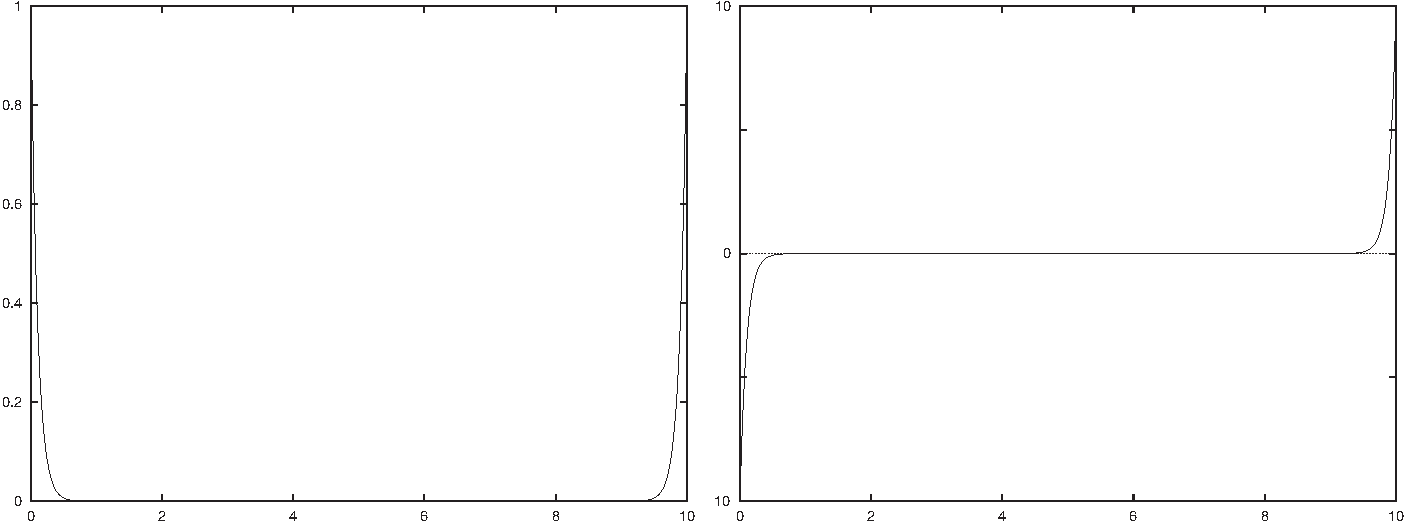
\includegraphics[width=0.98\textwidth]{matice}\\
\caption[]{Výsledek řešení úlohy (\ref{priklmetstr}), (\ref{priklOKP2}) metodou střelby na více cílů
(vlevo je hodnota funkce $x(t)$, vpravo její derivace $\dot x(t)$).}
\label{matice}
\end{figure}

%%% 10. prednaska 2004:
\subsection{Metoda sítí}

{\em Metoda sítí} (nebo {\em metoda konečných diferencí} či {\em diferenční metoda})
je založena na jednoduché myšlence diskretizace spojitého prostoru a převedení 
spojité diferenciální rovnice na soustavu algebraických rovnic nahrazením derivací 
přibližnými diferenčními vztahy. Výsledkem výpočtu je pak množina přibližných hodnot funkce
řešení v několika bodech prostoru.

Diskretizace prostoru se provádí konstrukcí tzv. {\em sítě}, tj. konečné množiny bodů
z intervalu $\langle a,b\rangle$, většinou, ne však nutně, ekvidistantně rozložených, tedy
obvykle množina 
\begin{equation}\label{sitFDM}
\{t_k=a+kh | k=0,\dots,n\}
\end{equation}
kde $h =(b-a)/n$ a $n$ je přirozené číslo.
Diskretizace rovnic se provádí nahrazením derivací tzv. {\em diferenčními podíly}, tedy 
vhodnými lineárními kombinacemi funkčních hodnot v bodech sítě. Tento postup vede 
k přeformulování úlohy řešení diferenciální rovnice v intervalu $\langle a,b\rangle$ na
úlohu řešení soustavy algebraických rovnic (v případě, že jde o řešení lineární 
diferenciální rovnice, je i výsledná soustava algebraických rovnic lineární).

V této kapitole se budeme věnovat především tomu, jak konstruovat diferenční podíly, 
jak určit jejich \uv{vhodnost} a jak interpretovat okrajové podmínky úlohy.

Dříve, než se budeme metodě věnovat hlouběji, uvedeme jednoduchý případ, pro který 
vybudujeme zcela intuitivně rovnice metody sítí. Řešme úlohu popsanou diferenciální 
rovnicí druhého řádu
\begin{equation}\label{prikFDM}
\ddot x=f(t,x),~~~~ t\in(a,b)
\end{equation}
s okrajovými podmínkami
\begin{equation}\label{OKPFDM}
x(a)=\gamma_1,~~~~ x(b)=\gamma_2.
\end{equation}
Tato úloha má za předpokladu, že je funkce $f$ hladká a její parciální derivace podle 
$x$ nezáporná, právě jedno řešení. Definujeme-li síť podle (\ref{sitFDM}) a nahradíme-li
druhou derivaci funkce $x$ v bodě $t_k$ podílem $\frac{x(t_{k+1})-2x(t_k)+x(t_{k-1})}{h^2}$,
dostaneme $n-1$ rovnic pro $n+1$ neznámých hodnot funkce $x$ ve tvaru
\begin{equation}\label{FDM1}
\frac{x(t_{k+1})-2x(t_k)+x(t_{k-1})}{h^2}=f(t_k,x(t_k))+\varepsilon_k,~~~~k=1,\dots,n-1,
\end{equation}
kde $\varepsilon_k$ je chyba přibližného diferenčního vzorce pro druhou derivaci.
Okrajové podmínky (\ref{OKPFDM}) doplňují soustavu o potřebné dvě rovnice. Vypuštěním
neznámé chyby $\varepsilon_k$ z rovnic (\ref{FDM1}) dostáváme soustavu $n+1$ (obecně
nelineárních) algebraických rovnic pro $n+1$ neznámých odhadů hodnot funkce $x$ 
v~bodech $t_k$, které označíme $x_k$:
\begin{equation}\label{FDM2}
\begin{array}{rcl}
x_{k+1}-2x_k+x_{k-1}&=&h^2 f(t_k,x_k),~~~~k=1,\dots,n-1,\\
x_0 &=&\gamma_1,\\
x_n &=&\gamma_2.
\end{array}
\end{equation}

Formálně jsme zkonstruovali rovnice (\ref{FDM2}) snadno. Abychom ale mohli mluvit
o numerické metodě, je třeba ověřit tři důležité vlastnosti soustavy (\ref{FDM2}):
\begin{enumerate}
\item Má soustava rovnic jednoznačné řešení?
\item Kterou metodu pro řešení soustav lineárních algebraických rovnic použít a jaká bude její přesnost?
\item Jaký je vztah mezi hodnotami $x_k$ a řešením původní diferenciální úlohy 
$x(t_k)$ při $h\to 0$?
\end{enumerate}
Obecný postup pro řešení těchto otázek zatím neexistuje. Je třeba ho pro každý typ úlohy 
provést zvlášť. Následující text se bude věnovat pouze třetímu z uvedených problémů a 
pouze pro jeden typ diferenciálních rovnic a okrajových podmínek.

\subsubsection{Konstrukce diferenčních vztahů}
Od diferenčních vztahů budeme přirozeně požadovat, aby konvergovaly k hodnotě derivace
pro $h$ klesající k nule. Výhodně pro jejich konstrukci můžeme využít větu o Taylorově 
rozvoji:
\begin{theorem}\label{TaylorV}
Buď funkce $x$ v intervalu $\langle a,b\rangle$ $(N+1)$-krát diferencovatelná a buďte $T$ 
číslo a $H$ nenulové reálné číslo tak, že $\langle T,T+H\rangle\subset\langle a,b\rangle$, 
resp. $\langle T+H,T\rangle\subset\langle a,b\rangle$. Pak existuje bod $\zeta\in(T,T+H)$, 
resp. $\zeta\in(T+H,T)$ takový, že
\begin{equation}\label{taylorV}
\begin{array}{rcl}
x(T+H)&=&\sum_{i=0}^{N} \frac{H^i}{i!} x^{(i)}(T)+\frac{H^{N+1}}{(N+1)!}x^{(N+1)}(\zeta)=\\
&=&x(T)+H\dot x(T)+\frac 12H^2\ddot x(T)+\frac 16H^3 x^{(3)}(T)+\dots+\\
&+&\frac{H^N}{N!}x^{(N)}(T)+\frac{H^{N+1}}{(N+1)!}x^{(N+1)}(\zeta).
\end{array}
\end{equation}
\end{theorem}

Pro dvakrát diferencovatelnou funkci $x$ tedy platí vztah
\begin{displaymath}
x(t+h)=x(t)+h\dot x(t)+\frac 12h^2\ddot x(\zeta),
\end{displaymath}
jehož jednoduchou úpravou dojdeme k prvnímu diferenčnímu vzorci 
pro první derivaci
\begin{equation}\label{DV1a}
\dot x(t)=\frac{x(t+h)-x(t)}h - \frac 12\ddot x(\zeta)h.
\end{equation}

Pro třikrát spojitě diferencovatelnou funkci $x$ můžeme zapsat 
vztahy
\begin{eqnarray*}
x(t+h)&=&x(t)+h\dot x(t)+\frac 12h^2\ddot x(t)+\frac 16h^3 x^{(3)}(\zeta_1),\\
x(t-h)&=&x(t)-h\dot x(t)+\frac 12h^2\ddot x(t)-\frac 16h^3 x^{(3)}(\zeta_2),
\end{eqnarray*}
jejichž odečtením, vydělením číslem $2h$ a použitím věty o střední hodnotě 
(která v tomto případě zaručuje existenci bodu $\zeta\in\langle t-h, t+h\rangle$
takového, že $\frac{x^{(3)}(\zeta_1)+X^{(3)}(\zeta_2)}2=x^{(3)}(\zeta)$) dostáváme jiný 
diferenční vztah pro první derivaci
\begin{equation}\label{DV1s}
\dot x(t)=\frac{x(t+h)-x(t-h)}{2h} - \frac 16x^{(3)}(\zeta)h^2.
\end{equation}

Pro čtyřikrát spojitě diferencovatelnou funkci $x$ můžeme zapsat 
vztahy
\begin{eqnarray*}
x(t+h)&=&x(t)+h\dot x(t)+\frac 12h^2 \ddot x(t)+\frac 16h^3x^{(3)}(t)+\frac 1{24}h^4x^{(4)}(\zeta_1),\\
x(t-h)&=&x(t)-h\dot x(t)+\frac 12h^2 \ddot x(t)-\frac 16h^3x^{(3)}(t)+\frac 1{24}h^4x^{(4)}(\zeta_2),
\end{eqnarray*}
jejichž sečtením, vydělením číslem $h^2$ a užitím věty o střední hodnotě 
dostaneme diferenční vztah pro druhou derivaci
\begin{equation}\label{DV2}
\ddot x(t)=\frac{x(t+h)-2x(t)+x(t-h)}{h^2} - \frac 1{12}x^{(4)}(\zeta)h^2.
\end{equation}

Diferenční podíl (\ref{DV1s}) lze odvodit také tak, že zkonstruujeme polynom 
2. stupně tak, že v bodech $t-h$, $t$, $t+h$ nabývá po řadě hodnot $x(t-h)$, $x(t)$, 
$x(t+h)$ a vyjádříme jeho derivaci v bodě $t$. Podobně lze odvodit ostatní dva 
uvedené diferenční vzorce a stejný postup lze aplikovat pro odvozování dalších 
diferenčních vzorců.

%%% 11. prednaska 2004:
\subsubsection{Lineární samoadjungovaná diferenciální rovnice}
Řešme lineární samoadjungovanou diferenciální rovnici druhého řádu 
(\ref{samoadj})
\begin{equation}\label{samoadj1}
-(p(t)\dot x)\dot{}+q(t)x=f(t)
\end{equation}
v intervalu $\langle a,b\rangle$
s lineárními separovanými okrajovými podmínkami
\begin{equation}\label{lsokp1}
\begin{array}{rcl}
-\alpha_1 p(a) \dot x(a) + \beta_1 x(a)&=&\gamma_1,\\
\alpha_2 p(b) \dot x(b) + \beta_2 x(b)&=&\gamma_2.
\end{array}
\end{equation}

Poznamenáme, že postačujícími, nikoliv nutnými, podmínkami jednoznačného řešení 
úlohy (\ref{samoadj1}), (\ref{lsokp1}) jsou
\begin{displaymath}
 p(t) \geq p_0 > 0~~~~~q(t) > 0~~~~~p,\dot p,q,f \mbox{~spojité}~~~~~\alpha_1 >0~~~~~\alpha_2 >0
\end{displaymath}

Rozdělíme interval $\langle a,b\rangle$ na $n$ dílků délky $h$ body sítě 
(\ref{sitFDM}) a budeme aproximovat operátor na levé straně rovnice 
(\ref{samoadj1})
\begin{equation}\label{opL}
\begin{array}{rcl}
(L x)(t)&=&-[p(t)\dot x(t)]\,\dot{}+q(t)x(t)\\
&=&-\dot p(t)\dot x(t)-p(t)\ddot x(t)+q(t)x(t)
\end{array}
\end{equation}
s užitím vzorců (\ref{DV1s}) a (\ref{DV2}) operátorem
\begin{equation}\label{opL0}
\begin{array}{rcl}
\left(L_h^{(0)} \vc x\right)_k&=&\frac 1{h^2}\Big\{-[p(t_k)-\frac 12 h\dot p(t_k)]x_{k-1}+\\
&+&[2p(t_k)+h^2q(t_k)]x_k-[p(t_k)+\frac 12 h\dot p(t_k)]x_{k+1}\Big\},
\end{array}
\end{equation}
kde $\vc x=(x_0,\dots,x_n)^T$ je vektor odhadů hodnot řešení rovnice 
(\ref{samoadj1}) v bodech sítě.

Vlastnosti použitých diferenčních podílů zaručují platnost následující věty:
\begin{theorem}\label{FDM-I}
Buď $p$, resp. $q$ v intervalu $\langle a,b\rangle$ spojitě diferencovatelná,
resp. spojitá a nechť má řešení úlohy (\ref{samoadj1}), (\ref{lsokp1}) $x$ 
v intervalu $\langle a,b\rangle$ čtyři spojité derivace. Označme 
$\vc x^{\ \rm(presny)}=(x(t_0),\dots,x(t_n))^T$. Potom platí
\begin{displaymath}
\left(L_h^{(0)} \vc x^{\ \rm(presny)}\right)_k = (Lx)(t_k)+O(h^2), ~~~~ k=1,\dots,n-1.
\end{displaymath}
\end{theorem}
{\bf Důkaz:}\nopagebreak
\begin{displaymath}
(Lx)(t_k) = -\dot p(t_k)\dot x(t_k)-p(t_k)\ddot x(t_k)+q(t_k)x(t_k)
\end{displaymath}
za předpokladu existence čtyř spojitých derivací funkce $x$ s užitím vzorců 
(\ref{DV1s}) a (\ref{DV2}) dostáváme přímo rovnost
\begin{eqnarray*}
(Lx)(t_k) &=& \frac 1{h^2}\Big\{-[p(t_k)-\frac 12 h\dot p(t_k)]x(t_{k-1})+[2p(t_k)+h^2q(t_k)]x(t_k)-\\
&-& [p(t_k)+\frac 12 h\dot p(t_k)]x(t_{k+1})\Big\}+O(h^2)=\\
&=& \left(L_h^{(0)} \vc x^{\ \rm(presny)}\right)_k + O(h^2)
\end{eqnarray*}
{\bf Q.E.D.}

~

Operátory levých stran okrajových podmínek (\ref{lsokp1})
\begin{eqnarray}\label{opl1}
l^{(1)} x&=&-\alpha_1 p(a) \dot x(a) + \beta_1 x(a),\\ \label{opl2}
l^{(2)} x&=&\alpha_2 p(b) \dot x(b) + \beta_2 x(b).
\end{eqnarray}
můžeme aproximovat pomocí diferenčního podílu (\ref{DV1a}) operátory
\begin{eqnarray}\label{opl1h}
l_h^{(1)} \vc x&=&-\alpha_1 p(a) \frac{x_1-x_0}h + \beta_1 x_0,\\ \label{opl2h}
l_h^{(2)} \vc x&=&\alpha_2 p(b) \frac{x_n-x_{n-1}}h + \beta_2 x_n,
\end{eqnarray}
kde $\vc x=(x_0,\dots,x_n)^T$ je vektor odhadů hodnot řešení rovnice.

Pro tuto aproximaci lze dokázat větu
\begin{theorem}\label{FDM-A}
Nechť $p$ je v intervalu $\langle a,b\rangle$ spojitá funkce a nechť má řešení 
úlohy (\ref{samoadj1}), (\ref{lsokp1}) $x$ v intervalu $\langle a,b\rangle$ 
dvě spojité derivace. $\vc x^{\ \rm(presny)}$ má stejný význam jako ve 
větě \ref{FDM-I}. Potom platí
\begin{displaymath}
l_h^{(1)} \vc x^{\ \rm(presny)} = l^{(1)}x+O(h), ~~~~~~~~~~
l_h^{(2)} \vc x^{\ \rm(presny)} = l^{(2)}x+O(h).
\end{displaymath}
\end{theorem}
{\bf Důkaz} vyplývá přímo ze vzorce (\ref{DV1a}) a předpokladu existence dvou
spojitých derivací funkce $x$.

Jsou-li složky vektoru $\vc x^{\ \rm(presny)}$ přesnými hodnotami řešení úlohy
(\ref{samoadj1}), (\ref{lsokp1}) postupně v bodech $t_0,\dots,t_n$, platí pro
ně podle vět \ref{FDM-I} a \ref{FDM-A} vztahy
\begin{displaymath}
\begin{array}{rcl}
\left(L_h^{(0)} \vc x^{\ \rm(presny)}\right)_k &=& f(t_k)+O(h^2), ~~~~~~~k=1,\dots,n-1\\
l_h^{(1)} \vc x^{\ \rm(presny)} &=& \gamma_1+O(h),\\
l_h^{(2)} \vc x^{\ \rm(presny)} &=& \gamma_2+O(h).
\end{array}
\end{displaymath}
Nabízí se tedy přímo jako rozumné hledat odhad řešení $x$ ze soustavy rovnic
\begin{equation}\label{IA}
\begin{array}{rcl}
\left(L_h^{(0)} \vc x\right)_k &=& f(t_k), ~~~~~~~k=1,\dots,n-1\\
l_h^{(1)} \vc x &=& \gamma_1,\\
l_h^{(2)} \vc x &=& \gamma_2.
\end{array}
\end{equation}

Pokud bychom chtěli tuto metodu použít, měli bychom ověřit řešitelnost soustavy 
(\ref{IA}) a konvergenci takto získaného odhadu řešení při $h\to 0$. My 
však nejprve poukážeme na jednu, na první pohled nepodstatnou, vadu takto 
získané soustavy. Diferenciální operátor levé strany rovnice (\ref{samoadj1}) 
$L$ definovaný vztahem (\ref{opL}) je samoadjungovaný. To by mělo umožňovat 
sestavení symetrické diferenční soustavy. Soustava (\ref{IA}) však symetrii 
neobsahuje (koeficient u neznámé $x_{k+1}$ v $k$-té rovnici $p(t_k)+\frac h2
\dot p(t_k)$ je pouze přibližně roven koeficientu u neznámé $x_k$ v $(k+1)$-ní
rovnici $p(t_{k+1})-\frac h2 \dot p(t_{k+1})$).

%%% 12. prednaska 2004:
Symetrii lze zachovat využitím samoadjungovanosti operátoru $L$ tak, že 
derivace nahradíme diferenčními vzorci už v prvním řádku vztahu (\ref{opL}). 
Tedy nejprve označíme součin $p(t)\dot x(t)$ symbolem $z(t)$ a nahradíme v prvním
členu derivaci $\dot z(t)$ diferenčním vzorcem (\ref{DV1s}) s polovičním krokem, 
tj. podílem $[z(t_k+\frac h2)-z(t_k-\frac h2)]/h$. Po zpětném dosazení 
původního součinu za $z(t)$ nahradíme první derivace $\dot x(t_k-\frac h2)$ a
$\dot x(t_k+\frac h2)$ podle téhož vzorce s polovičním krokem a dostaneme 
diskrétní operátor $L_h$ ve tvaru
\begin{equation}\label{opLh}
\begin{array}{rcl}
(L_h \vc x)_k&=&\frac 1{h^2}\Big\{-p(t_k-\frac h2)x_{k-1}+\\
&+&[p(t_k-\frac h2)+p(t_k+\frac h2)+h^2q(t_k)]x_k-p(t_k-\frac h2)x_{k+1}\Big\}.
\end{array}
\end{equation}

Ten má podobné vlastnosti jako operátor $L_h^{(0)}$, což přesněji vyjadřuje 
následující věta:
\begin{theorem}\label{FDM-II}
Buď $p$, resp. $q$ v intervalu $\langle a,b\rangle$ třikrát spojitě diferencovatelná,
resp. spojitá a nechť má řešení úlohy (\ref{samoadj1}), (\ref{lsokp1}) $x$ 
v intervalu $\langle a,b\rangle$ čtyři spojité derivace. Označme 
$\vc x^{\ \rm(presny)}=(x(t_0),\dots,x(t_n))^T$. Potom platí
\begin{displaymath}
(L_h \vc x^{\ \rm(presny)})_k = (Lx)(t_k)+O(h^2), ~~~~ k=1,\dots,n-1.
\end{displaymath}
\end{theorem}
{\bf Důkaz:}
Důkaz nelze provést přímo z vlastností vzorce (\ref{DV1s}), jako v případě Věty \ref{FDM-I}.
Provedeme jej v několika krocích:
\begin{enumerate}
\item
Z Taylorova rozvoje v bodě $t+\frac h2$ hodnot funkce $x$ se čtyřmi spojitě 
diferencovatelnými derivacemi v bodech $t+h$ a $t$ dostáváme rovnice:
\begin{eqnarray*}
 x(t+h) &=& x(t+\frac h2) + \frac h2 \dot x(t+\frac h2) + \frac 12 \left(\frac h2\right)^2 \ddot x(t+\frac h2) +\\
 &+& \frac 16 \left(\frac h2\right)^3 x^{(3)}(t+\frac h2) + O(h^4),\\
 x(t)   &=& x(t+\frac h2) - \frac h2 \dot x(t+\frac h2) + \frac 12 \left(\frac h2\right)^2 \ddot x(t+\frac h2) -\\
 &-& \frac 16 \left(\frac h2\right)^3 x^{(3)}(t+\frac h2) + O(h^4),
\end{eqnarray*}
jejichž vzájemným odečtením dostaneme rovnost
\begin{equation}\label{duk1-a}
 x(t+h) - x(t) = h \dot x(t+\frac h2) + \frac 1{24} h^3 x^{(3)}(t+\frac h2) + O(h^4).
\end{equation}
\item
Podobně odečtením Taylorových rozvojů v bodě $t-\frac h2$ hodnot funkce $x$ 
v~bodech $t$ a $t-h$ dostaneme rovnost
\begin{equation}\label{duk1-b}
 x(t) - x(t-h) = h \dot x(t-\frac h2) + \frac 1{24} h^3 x^{(3)}(t-\frac h2) + O(h^4).
\end{equation}
Rozdíl rovnice (\ref{duk1-a}) vynásobené hodnotou $\frac{p(t+ \frac h2)}{h^2}$
a rovnice (\ref{duk1-b}) vynásobené hodnotou $\frac{p(t- \frac h2)}{h^2}$ dává
vztah:
\begin{equation}\label{duk1}
\begin{array}{l}
 \frac 1{h^2}\left[p(t+\frac h2) (x(t+h) - x(t))- p(t-\frac h2) (x(t) - x(t-h))\right] = \\
 = \frac {p(t+\frac h2)\dot x(t+\frac h2)-p(t-\frac h2)\dot x(t-\frac h2)}{h} + \\
 + \frac 1{24} h\left[p(t+\frac h2) x^{(3)}(t+\frac h2)-p(t-\frac h2) x^{(3)}(t-\frac h2)\right] + O(h^2).
\end{array}
\end{equation}
\item
Pro libovolnou třikrát spojitě diferencovatelnou funkci $z$ platí podle (\ref{DV1s})
rovnost
\begin{equation}\label{duk2-a}
 \frac{z(t+\frac h2)-z(t- \frac h2)}{h} = \dot z(t)+O(h^2).
\end{equation}
Dosadíme-li vzorec (\ref{duk2-a}) pro funkci $z(t)=p(t)\dot x(t)$ do rovnice (\ref{duk1}),
vynásobíme celou rovnici číslem $-1$ a přičteme-li k oběma stranám rovnice člen 
$q(t)x(t)$, můžeme psát
\begin{equation}\label{duk2}
\begin{array}{l}
 \frac {-p(t+\frac h2)x(t+h) + \left(p(t+\frac h2)+p(t-\frac h2)+h^2q(t)\right) x(t)- p(t-\frac h2) x(t-h)}{h^2} =\\
 =-(p(t)\dot x(t))\dot{}+ q(t)x(t)-\\
 - \frac 1{24} h\left[p(t+\frac h2) x^{(3)}(t+\frac h2)-p(t-\frac h2) x^{(3)}(t-\frac h2)\right] + O(h^2).
\end{array}
\end{equation}
\item 
Taylorův rozvoj v bodě $t-\frac h2$ hodnoty spojitě diferencovatelné funkce $w$ 
v bodě $t+\frac h2$ můžeme psát ve tvaru:
\begin{displaymath}
 w(t+\frac h2)=w(t-\frac h2) + h \dot w(\zeta),
\end{displaymath}
kde $\zeta\in\langle t-\frac h2; t+\frac h2\rangle\subset\langle a, b\rangle$.
Navíc funkce $\dot w$ spojitá na uzavřeném intervalu $\langle a, b\rangle$ musí být
omezená. Označme $M$ číslo omezující hodnoty $\dot w$ v intervalu $\langle a, b\rangle$
(tedy $(\forall t\in\langle a,b\rangle)(|\dot w(t)|<M)$ a můžeme psát
\begin{equation}\label{duk3-a}
 |w(t+\frac h2)-w(t-\frac h2)| < h M.
\end{equation}
Zvolíme-li konkrétně funkci $w(t)=p(t)x^{(3)}(t)$, říká rovnost (\ref{duk3-a}):
\begin{displaymath}
 \frac 1{24} h\left[p(t+\frac h2) x^{(3)}(t+\frac h2)-p(t-\frac h2) x^{(3)}(t-\frac h2)\right] = O(h^2),
\end{displaymath}
a odtud a z rovnice (\ref{duk2}) vyplývá přímo tvrzení věty.
\end{enumerate}
{\bf Q.E.D.}

~

Jejím důsledkem je návrh dalšího systému algebraických rovnic pro aproximaci řešení 
původní úlohy:
\begin{equation}\label{IIA}
\begin{array}{rcl}
(L_h \vc x)_k &=& f(t_k), ~~~~~~~k=1,\dots,n-1\\
l_h^{(1)} \vc x &=& \gamma_1,\\
l_h^{(2)} \vc x &=& \gamma_2.
\end{array}
\end{equation}
Vynásobíme-li poslední dvě rovnice aproximující okrajové podmínky vhodnými 
konstantami a přesuneme-li předposlední rovnici v systému na první místo, 
je výsledná soustava symetrická. O tomto systému lze dokázat, že má 
jediné řešení (pokud byla úloha (\ref{samoadj1}), (\ref{lsokp1}) jednoznačně
řešitelná) a jeho konvergenční vlastnosti shrnuje následující věta:
\begin{theorem}\label{V3.7}
Nechť má úloha (\ref{samoadj1}), (\ref{lsokp1}) jednoznačné řešení a nechť
je navíc funkce $p$ v intervalu $\langle a,b\rangle$ třikrát spojitě 
diferencovatelná a funkce $q$ a $f$ dvakrát spojitě diferencovatelné. 
Buď dále $x_k$ přibližné řešení vypočtené ze soustavy (\ref{IIA}). Pak 
existují konstanty $M$ a $h_0>0$ tak, že pro každé $h<h_0$ platí
\begin{displaymath}
|x_k-x(t_k)|\leq Mh, ~~~~~~~~~~~~~ k=0,\dots, n.
\end{displaymath}
\end{theorem}
Rychlost konvergence je tedy $O(h)$, ačkoliv operátor $L$ je o řád 
přesnější. Nižší přesnost operátorů $l_h^{(1)}$ a $l_h^{(2)}$ převážila.
Na jednoduchém příkladu si ukážeme, že obecně nelze rychlost konvergence 
omezit nijak silněji:

Řešme rovnici 
\begin{equation}\label{uloha1}
\ddot x(t)=2~~~~~~~~~~~~~~\Leftrightarrow~~~~~~~~~~~~~~-\ddot x(t)=-2
\end{equation}
v intervalu $t\in\langle -1;1\rangle$ 
s okrajovými podmínkami 
\begin{equation}\label{uloha2}
\begin{array}{rcl}
-\dot x(-1)+x(-1)&=&3,\\
\dot x(1)+x(1)&=&3.
\end{array}
\end{equation}
Zadání odpovídá úloze (\ref{samoadj1}), (\ref{lsokp1}) s parametry $p(t)\equiv 1$,
$q(t)\equiv 0$, $f(t)\equiv -2$, $\alpha_1=\alpha_2=\beta_1=\beta_2=1$, 
$\gamma_1=\gamma_2=3$. Její přesné řešení má tvar $x(t)=t^2$. Diferenční rovnice 
(\ref{IIA}) pro uvedenou úlohu mají tvar
\begin{displaymath}
\begin{array}{rcl}
-x_{k-1}+2x_k-x_{k+1} &=& -2h^2,~~~~~~~~k=1,\dots,n-1\\
-\frac{x_1-x_0}h+x_0&=& 3,\\
\frac{x_n-x_{n-1}}h+x_n&=& 3
\end{array}
\end{displaymath}
a jejich řešením je vektor o složkách $x_k=t_k^2+h$.

Chyba řešení je tedy {\em přesně} $h$ a to v celém intervalu, nejen na 
krajích intervalu. Tuto poznámku uvádíme proto, že úvaha o převážení nižší
přesnosti operátorů $l_h^{(1)}$ a $l_h^{(2)}$ nad vyšší přesností operátoru
$L_h$ vede k očekávání, že řešení bude přesnější uvnitř intervalu než na 
jeho krajích. Tato představa se alespoň v tomto konkrétním případě nepotvrzuje 
-- chyba se přenáší po celé šířce intervalu.

%%% 13. prednaska 2004:
Příklad nás vede k myšlence aproximovat přesnějšími diferenčními vztahy 
okrajové podmínky. Potíž je však v tom, že okrajové podmínky jsou předepisovány 
na okraji řešeného intervalu a nemáme tudíž k dispozici odhady řešení na obou 
stranách od krajního bodu. Musíme tedy pro odhad používat pouze informace 
z jedné strany, což komplikuje tvorbu přesnějších diferenčních vztahů. Ty,
které tato problematika zaujala, nebo podobný problém řeší, odkážeme na 
knihu \cite{Vit}. Zde jako motivaci uvedeme bez odvozování pouze jeden typ 
odhadu okrajových podmínek (\ref{lsokp1}) a jeho vlastnosti. Definujme nové 
dva operátory
\begin{eqnarray}\label{opl1dh}
l_h^{(1,\d)} \vc x&=&-\alpha_1 p(a+\frac h2) \frac{x_1-x_0}h + [\frac 12\alpha_1 hq(a)+\beta_1]x_0,\\ \label{opl2dh}
l_h^{(2,\d)} \vc x&=&\alpha_2 p(b-\frac h2) \frac{x_n-x_{n-1}}h + [\frac 12\alpha_2 hq(b)+\beta_2]x_n.
\end{eqnarray}
Pro ně lze dokázat větu:
\begin{theorem}\label{FDM-B}
Nechť $p$ je v intervalu $\langle a,b\rangle$ dvakrát spojitě diferencovatelná 
a funkce $q$ spojitá. Nechť má řešení úlohy (\ref{samoadj1}), (\ref{lsokp1}) 
$x$ v intervalu $\langle a,b\rangle$ tři spojité derivace. 
$\vc x^{\ \rm(presny)}$ má stejný význam jako ve větě \ref{FDM-II}. Potom platí
\begin{eqnarray*}
l_h^{(1,\d)} \vc x^{\ \rm(presny)} &=& l^{(1)}x+ \frac 12\alpha_1 h(Lx)(a)+O(h^2),\\
l_h^{(2,\d)} \vc x^{\ \rm(presny)} &=& l^{(2)}x+ \frac 12\alpha_2 h(Lx)(b)+O(h^2).
\end{eqnarray*}
\end{theorem}

Pro (po přenásobení posledních dvou rovnic vhodnými konstantami a přeuspořádání) 
symetrický systém diferenčních rovnic 
\begin{equation}\label{IIB}
\begin{array}{rcl}
(L_h \vc x)_k &=& f(t_k),~~~~~~~~k=1,\dots,n-1\\
l_h^{(1,\d)} \vc x &=& \gamma_1 + \frac 12\alpha_1 hf(a),\\
l_h^{(2,\d)} \vc x &=& \gamma_2 + \frac 12\alpha_2 hf(b)
\end{array}
\end{equation}
pak platí věta:
\begin{theorem}\label{V3.9}
Nechť má úloha (\ref{samoadj1}), (\ref{lsokp1}) jednoznačné řešení a nechť
je navíc funkce $p$ v intervalu $\langle a,b\rangle$ třikrát spojitě 
diferencovatelná a funkce $q$ a $f$ dvakrát spojitě diferencovatelné. 
Buď dále $x_k$ přibližné řešení vypočtené ze soustavy (\ref{IIB}). Pak 
existují konstanty $M$ a $h_0>0$ tak, že pro každé $h<h_0$ platí
\begin{displaymath}
|x_k-x(t_k)|\leq Mh^2, ~~~~~~~~~~~~~ k=0,\dots, n.
\end{displaymath}
\end{theorem}

Vraťme se k příkladu (\ref{uloha1}), (\ref{uloha2}). Diferenční rovnice 
(\ref{IIB}) pro jeho přibližné řešení mají tvar
\begin{displaymath}
\begin{array}{rcl}
-x_{k-1}+2x_k-x_{k+1} &=& -2h^2,~~~~~~~~k=1,\dots,n-1\\
-\frac{x_1-x_0}h+x_0&=& 3 - h  ,\\
\frac{x_n-x_{n-1}}h+x_n&=& 3 - h
\end{array}
\end{displaymath}
a jejich řešením je vektor o složkách $x_k=t_k^2$. Přibližné řešení díky
tomu, že přesné řešení má tvar paraboly, dokonce přesně vystihuje hodnoty
v uzlových bodech sítě.

Závěrem se zamyslíme nad tím, jak lze obecně zvyšovat rychlost konvergence 
metody sítí (a tím dosahovat menší diskretizační chyby při hrubější diskretizaci 
a tím urychlovat výpočet a zlepšovat jeho mezní přesnost). Zjevně vede cesta 
nahrazením derivací přesnějšími diferenčními podíly. Přesnější diferenční podíly 
můžeme odvozovat jako derivace interpolačních polynomů vyšších řádů. Pro proložení 
funkce polynomem vyššího řádu je ale třeba znát více funkčních hodnot, proto 
v těchto vzorcích budou vystupovat hodnoty hledané funkce ve více uzlech sítě.
Například dvojím derivováním interpolačního polynomu čtvrtého stupně dostaneme 
následující symetrickou aproximaci druhé derivace:
\begin{displaymath}
\ddot x(t_k)=\frac{-x(t_{k-2})+16x(t_{k-1})-30x(t_k)+16x(t_{k+1})-x(t_{k+2})}{12h^2}+O(h^4).
\end{displaymath}
Jeho výhodou je jeho vysoká přesnost. Jeho nevýhodami jsou větší složitost 
matice systému rovnic s jeho použitím sestavených (nebudou tridiagonální, ale 
pětidiagonální) a náročnost na okrajové podmínky. Tento vzorec bude možno aplikovat 
jen pro $k=2,\dots,n-2$. Dvě okrajové podmínky pak budou muset dodat do systému
čtyři rovnice. Navíc bude třeba najít takové interpolační vzorce pro okrajové
podmínky, aby neredukovaly vysokou přesnost zvoleného vzorce. Řešení obou 
problémů je obecně velmi náročné a zde skončíme pouze poukázáním na jeho existenci
a odkazem do publikací věnovaných metodě sítí.

% Formulace Cuachyovy úlohy pro soustavu prvního řádu 
% zavedeni vektorove notace
% example zapisu oscilatoru a dravec-korist
% autonomní rovnice

% prevod rovnic vyssiho radu na soustavy prvniho radu obecne
% typy soustav rovnic: linearni , nelinearni, konst. / nekonst. koeficienty


% theorem o exisenci reseni

% jednoznačnost řešení
% example nejednoznacnosti
% Lipschicovskost pro systemy
% exampley Lipsch a neLipsch funkci a systemu
% theorem o jednoznacnosti
% example neexistence a nejednoznacnosti

% stabilita bodu




\chapter{Numerické metody pro soustavy ODR}

\section{Explicitní Eulerova metoda}
% zminka o pouziti pro dukaz existence
\subsection{Chyba diskretizace}
\subsection{Lokální chyba metody}
\subsection{Globální chyba metody}
\subsection{Vliv zaokrouhlovacích chyb}
% optimalni krok pro konecnou presnost
\subsection{Oblast absolutní stability}
% theorem stabilita & konzistence => konvergence

\section{Implicitní Eulerova metoda}
\subsection{Stiff problémy}
\subsection{Oblast absolutní stability}
\subsection{Řešení nelineárních soustav}

\section{Rungeovy-Kuttovy metody}
\subsection{Metody druhého řádu}
\subsection{Obecná RK metoda}


\section{Vícekrokové metody}

\section{Adaptivní metody}
% metoda polovicniho kroku
% porovnani metod ruznych radu

\section{Přehled metod}

\section{Okrajové úlohy a metoda sítí}
\end{document}
